% Options for packages loaded elsewhere
\PassOptionsToPackage{unicode}{hyperref}
\PassOptionsToPackage{hyphens}{url}
%
\documentclass[
]{article}
\usepackage{lmodern}
\usepackage{amssymb,amsmath}
\usepackage{ifxetex,ifluatex}
\ifnum 0\ifxetex 1\fi\ifluatex 1\fi=0 % if pdftex
  \usepackage[T1]{fontenc}
  \usepackage[utf8]{inputenc}
  \usepackage{textcomp} % provide euro and other symbols
\else % if luatex or xetex
  \usepackage{unicode-math}
  \defaultfontfeatures{Scale=MatchLowercase}
  \defaultfontfeatures[\rmfamily]{Ligatures=TeX,Scale=1}
\fi
% Use upquote if available, for straight quotes in verbatim environments
\IfFileExists{upquote.sty}{\usepackage{upquote}}{}
\IfFileExists{microtype.sty}{% use microtype if available
  \usepackage[]{microtype}
  \UseMicrotypeSet[protrusion]{basicmath} % disable protrusion for tt fonts
}{}
\makeatletter
\@ifundefined{KOMAClassName}{% if non-KOMA class
  \IfFileExists{parskip.sty}{%
    \usepackage{parskip}
  }{% else
    \setlength{\parindent}{0pt}
    \setlength{\parskip}{6pt plus 2pt minus 1pt}}
}{% if KOMA class
  \KOMAoptions{parskip=half}}
\makeatother
\usepackage{xcolor}
\IfFileExists{xurl.sty}{\usepackage{xurl}}{} % add URL line breaks if available
\IfFileExists{bookmark.sty}{\usepackage{bookmark}}{\usepackage{hyperref}}
\hypersetup{
  pdftitle={Supplementary Information: Global patterns of forest autotrophic carbon fluxes},
  pdfauthor={Rebecca Banbury Morgan; Valentine Herrmann; Norbert Kunert; Ben Bond-Lamberty; Helene C. Muller-Landau; Kristina J. Anderson-Teixeira},
  hidelinks,
  pdfcreator={LaTeX via pandoc}}
\urlstyle{same} % disable monospaced font for URLs
\usepackage[margin=1in]{geometry}
\usepackage{graphicx,grffile}
\makeatletter
\def\maxwidth{\ifdim\Gin@nat@width>\linewidth\linewidth\else\Gin@nat@width\fi}
\def\maxheight{\ifdim\Gin@nat@height>\textheight\textheight\else\Gin@nat@height\fi}
\makeatother
% Scale images if necessary, so that they will not overflow the page
% margins by default, and it is still possible to overwrite the defaults
% using explicit options in \includegraphics[width, height, ...]{}
\setkeys{Gin}{width=\maxwidth,height=\maxheight,keepaspectratio}
% Set default figure placement to htbp
\makeatletter
\def\fps@figure{htbp}
\makeatother
\setlength{\emergencystretch}{3em} % prevent overfull lines
\providecommand{\tightlist}{%
  \setlength{\itemsep}{0pt}\setlength{\parskip}{0pt}}
\setcounter{secnumdepth}{-\maxdimen} % remove section numbering
\usepackage{float} \usepackage{caption} \captionsetup[table]{font=footnotesize} \captionsetup[figure]{font=footnotesize} \captionsetup[figure]{labelformat=empty} \captionsetup[table]{labelformat=empty} \usepackage{pdflscape} \newcommand{\blandscape}{\begin{landscape}} \newcommand{\elandscape}{\end{landscape}}
\usepackage{booktabs}
\usepackage{longtable}
\usepackage{array}
\usepackage{multirow}
\usepackage{wrapfig}
\usepackage{float}
\usepackage{colortbl}
\usepackage{pdflscape}
\usepackage{tabu}
\usepackage{threeparttable}
\usepackage{threeparttablex}
\usepackage[normalem]{ulem}
\usepackage{makecell}
\usepackage{xcolor}

\title{Supplementary Information: Global patterns of forest autotrophic carbon
fluxes}
\author{Rebecca Banbury Morgan \and Valentine Herrmann \and Norbert Kunert \and Ben Bond-Lamberty \and Helene C. Muller-Landau \and Kristina J. Anderson-Teixeira}
\date{}

\begin{document}
\maketitle

\listoftables
\listoffigures

\newpage

\begin{landscape}

\begin{table}[!h]

\caption{\label{tab:unnamed-chunk-2}Table S1. Climate variable definitions, sources, and abbreviations}
\centering
\resizebox{\linewidth}{!}{
\begin{tabular}[t]{>{\raggedright\arraybackslash}p{2.5cm}>{\raggedright\arraybackslash}p{5cm}>{\raggedright\arraybackslash}p{2cm}>{\raggedright\arraybackslash}p{7cm}>{\raggedright\arraybackslash}p{2cm}>{\raggedright\arraybackslash}p{5cm}}
\toprule
Abbreviation & Climate variable & Units & Definition & Time span & Source\\
\midrule
MAT & Mean annual temperature & $^\circ$C & Annual mean temperature, from primary literature or WorldClim if not reported & 1970 - 2000 & Primary literature; WorldClim$^{1}$\\
MAP & Mean annual precipitation & mm yr$^{-1}$ & Annual mean precipitation, from primary literature or WorldClim if not reported & 1970 - 2000 & Primary literature; WorldClim$^{1}$\\
T Seas & Temperature seasonality & $^\circ$C & Standard deviation (variation) of monthly temperature averages & 1970 - 2000 & WorldClim$^{1}$\\
P Seas & Precipitation seasonality & $\%$ & Coefficient of variation of mean monthly precipitation x 100 & 1970 - 2000 & WorldClim$^{1}$\\
ATR & Annual temperature range & $^\circ$C & Maximum temperature of warmest month - minimum temperature of coldest month & 1970 - 2000 & WorldClim$^{1}$\\
\addlinespace
Solar R & Solar radiation & kJ m$^{-2}$ yr$^{-1}$ & Solar radiation & 1970 - 2000 & WorldClim2$^{2}$\\
Cloud & Cloud cover & $\%$ & Cloud percentage cover & 1901 - 2014 & CRU time-series dataset v 4.03$^{3}$\\
AFD & Annual frost days & days yr$^{-1}$ & Number of freeze days annually & 1901 - 2014 & CRU time-series dataset v 4.03$^{3}$\\
AWD & Annual wet days & days yr$^{-1}$ & Number of days with precipitation >0.1 mm annually & 1901 - 2014 & CRU time-series dataset v 4.03$^{3}$\\
PET & Potential evapotranspiration & mm yr$^{-1}$ & Mean annual potential evapotranspiration & 1950 - 2000 & Global Aridity Index and Potential Evapotranspiration Climate Database$^{4}$\\
\addlinespace
AI & Aridity &  & MAP/mean annual PET & 1950 - 2000 & Global Aridity Index and Potential Evapotranspiration Climate Database$^{4}$\\
VPD & Vapour pressure deficit & kPa & Mean monthly vapour pressure deficit & 1958 - 2015 & TerraClimate$^{5}$\\
Max VPD & Maximum vapour pressure deficit & kPa & Maximum monthly vapour pressure deficit & 1958 - 2017 & Derived from TerraClimate data\\
WSM & Water stress months & months yr$^{-1}$ & Number of months annually with MAP < PET & 1970 - 2000 & Derived from WorldClim data\\
LGS & Length of growing season & months yr$^{-1}$ & Number of months annually with mean minimum temperature > 0.5$^\circ$C & 1901 - 2014 & Derived from CRU data\\
\addlinespace
gsT & Growing season temperature & $^\circ$C & Mean growing season temperature & 1901 - 2014 & Derived from CRU data\\
gsP & Growing season precipitation & mm month$^{-1}$ & Mean monthly precipitation during growing season months & 1901 - 2014 & Derived from CRU data\\
gsPET & Growing season PET & mm month$^{-1}$ & Mean monthly potential evapotranspiration during growing season months & 1901 - 2014 & Derived from CRU data\\
gsR & Growing season solar radiation & mm month$^{-1}$ & Mean monthly solar radiation during growing season & 1901 - 2014 & Derived from WorldClim2 data\\
\bottomrule
\multicolumn{6}{l}{\textsuperscript{*} The WorldClim version used was the most recent available at the time of analysis}\\
\multicolumn{6}{l}{\textsuperscript{1} Hijmans et al. (2005) \textsuperscript{2} Fick et al. (2017) \textsuperscript{3} Harris et al. (2017) \textsuperscript{4} Abatzoglou et al. (2018)}\\
\end{tabular}}
\end{table}
\end{landscape}
\newpage

\begin{landscape}
\begin{table}[!h]

\caption[Table S2. Model form, $\Delta$AIC and R$^{2}$ for each climate variables as a single fixed effect in models for each C flux]{\label{tab:unnamed-chunk-3}Table S2. Model form, $\Delta$AIC, and R$^{2}$ for each climate variable as a single fixed effect in models for each C flux.}
\centering
\resizebox{\linewidth}{!}{
\begin{tabular}[t]{llrrlrrlrrlrrllllrrllllll}
\toprule
\multicolumn{1}{c}{ } & \multicolumn{3}{c}{Latitude} & \multicolumn{3}{c}{MAT} & \multicolumn{3}{c}{MAP} & \multicolumn{3}{c}{T Seas} & \multicolumn{3}{c}{P Seas} & \multicolumn{3}{c}{ATR} & \multicolumn{3}{c}{Solar R} & \multicolumn{3}{c}{AI} \\
\cmidrule(l{3pt}r{3pt}){2-4} \cmidrule(l{3pt}r{3pt}){5-7} \cmidrule(l{3pt}r{3pt}){8-10} \cmidrule(l{3pt}r{3pt}){11-13} \cmidrule(l{3pt}r{3pt}){14-16} \cmidrule(l{3pt}r{3pt}){17-19} \cmidrule(l{3pt}r{3pt}){20-22} \cmidrule(l{3pt}r{3pt}){23-25}
Carbon Flux & Model & R$^{2}$ & $\Delta$ AIC & Model & R$^{2}$ & $\Delta$ AIC & Model & R$^{2}$ & $\Delta$ AIC & Model & R$^{2}$ & $\Delta$ AIC & Model & R$^{2}$ & $\Delta$ AIC & Model & R$^{2}$ & $\Delta$ AIC & Model & R$^{2}$ & $\Delta$ AIC & Model & R-sq & dAIC\\
\midrule
GPP & Lin & 0.64 & 54.9 & Lin & 0.61 & 52.5 & Lin & 0.18 & 33.3 & Poly & 0.71 & 69.5 & - & - & - & Poly & 0.69 & 63.0 & Log & 0.16 & 8.9 & - & - & -\\
NPP & Log & 0.50 & 44.3 & Lin & 0.42 & 41.5 & Poly & 0.21 & 16.7 & Log & 0.52 & 44.3 & - & - & - & Log & 0.49 & 42.3 & Poly & 0.16 & 12.5 & Lin & 0.04 & 2.8\\
ANPP & Lin & 0.44 & 63.4 & Lin & 0.44 & 80.5 & Poly & 0.16 & 19.7 & Log & 0.41 & 58.7 & - & - & - & Log & 0.37 & 51.9 & Lin & 0.11 & 12.3 & Lin & 0.05 & 2.1\\
ANPP stem & Lin & 0.18 & 22.2 & Lin & 0.24 & 38.5 & Log & 0.05 & 7.3 & Lin & 0.14 & 17.6 & Poly & 0.05 & 5 & Lin & 0.12 & 13.6 & Log & 0.06 & 6.8 & Lin & 0.07 & 4\\
ANPP foliage & Lin & 0.50 & 37.7 & Lin & 0.58 & 52.9 & Poly & 0.25 & 13.3 & Lin & 0.48 & 34.1 & - & - & - & Lin & 0.50 & 36.1 & Log & 0.17 & 10.1 & Lin & 0.11 & 6.8\\
\addlinespace
BNPP root & Lin & 0.34 & 22.9 & Log & 0.31 & 21.0 & Poly & 0.15 & 6.2 & Log & 0.36 & 26.6 & - & - & - & Log & 0.33 & 23.6 & Poly & 0.29 & 18.8 & - & - & -\\
BNPP fine root & Lin & 0.17 & 8.0 & Lin & 0.15 & 7.2 & Log & 0.11 & 5.4 & Lin & 0.17 & 8.4 & - & - & - & Log & 0.19 & 10.9 & Log & 0.14 & 7.2 & Log & 0.06 & 2.4\\
R auto & Lin & 0.65 & 13.1 & Lin & 0.59 & 10.9 & Poly & 0.60 & 8.6 & Log & 0.65 & 13.1 & - & - & - & Log & 0.60 & 11.5 & Log & 0.27 & 2.4 & Poly & 0.48 & 3.7\\
R root & Log & 0.22 & 8.8 & Lin & 0.24 & 8.3 & Lin & 0.15 & 6.8 & Log & 0.24 & 9.5 & - & - & - & Log & 0.22 & 8.8 & - & - & - & Lin & 0.16 & 7.3\\
\bottomrule
\end{tabular}}
\end{table}

\begin{table}[!h]
\centering
\resizebox{\linewidth}{!}{
\begin{tabular}{lllllrrllllrrlrrlllllllrr}
\toprule
\multicolumn{1}{c}{ } & \multicolumn{3}{c}{Cloud} & \multicolumn{3}{c}{AFD} & \multicolumn{3}{c}{AWD} & \multicolumn{3}{c}{PET} & \multicolumn{3}{c}{VPD} & \multicolumn{3}{c}{Max VPD} & \multicolumn{3}{c}{WSM} & \multicolumn{3}{c}{LGS} \\
\cmidrule(l{3pt}r{3pt}){2-4} \cmidrule(l{3pt}r{3pt}){5-7} \cmidrule(l{3pt}r{3pt}){8-10} \cmidrule(l{3pt}r{3pt}){11-13} \cmidrule(l{3pt}r{3pt}){14-16} \cmidrule(l{3pt}r{3pt}){17-19} \cmidrule(l{3pt}r{3pt}){20-22} \cmidrule(l{3pt}r{3pt}){23-25}
Carbon Flux & Model & R$^{2}$ & $\Delta$ AIC & Model & R$^{2}$ & $\Delta$ AIC & Model & R$^{2}$ & $\Delta$ AIC & Model & R$^{2}$ & $\Delta$ AIC & Model & R$^{2}$ & $\Delta$ AIC & Model & R$^{2}$ & $\Delta$ AIC & Model & R$^{2}$ & $\Delta$ AIC & Model & R$^{2}$ & $\Delta$ AIC\\
\midrule
GPP & - & - & - & Log & 0.54 & 50.0 & Lin & 0.11 & 5.7 & Poly & 0.36 & 19.7 & Poly & 0.31 & 15.9 & - & - & - & - & - & - & Lin & 0.53 & 38.2\\
NPP & Lin & 0.06 & 3.6 & Lin & 0.40 & 38.5 & Lin & 0.11 & 7.3 & Poly & 0.32 & 24.3 & Poly & 0.18 & 15.3 & - & - & - & Lin & 0.04 & 4 & Lin & 0.38 & 28.4\\
ANPP & Poly & 0.09 & 7.1 & Log & 0.41 & 61.6 & Lin & 0.17 & 18.7 & Poly & 0.27 & 24.5 & Poly & 0.23 & 21.4 & Poly & 0.06 & 2.2 & Poly & 0.06 & 3 & Lin & 0.34 & 44.0\\
ANPP stem & Poly & 0.09 & 5.4 & Log & 0.17 & 22.3 & - & - & - & Poly & 0.20 & 14.0 & Poly & 0.21 & 17.7 & Log & 0.14 & 7.5 & - & - & - & Log & 0.11 & 12.6\\
ANPP foliage & - & - & - & Lin & 0.53 & 43.4 & Lin & 0.15 & 7 & Log & 0.32 & 24.2 & Log & 0.35 & 30.0 & Poly & 0.07 & 4.9 & Poly & 0.17 & 7.8 & Log & 0.46 & 32.9\\
\addlinespace
BNPP root & - & - & - & Lin & 0.28 & 19.1 & Poly & 0.11 & 3.4 & Poly & 0.36 & 23.2 & Poly & 0.26 & 13.9 & - & - & - & - & - & - & Lin & 0.26 & 14.7\\
BNPP fine root & - & - & - & Lin & 0.16 & 9.2 & Lin & 0.08 & 2.7 & Log & 0.14 & 7.1 & Log & 0.06 & 1.9 & - & - & - & - & - & - & Lin & 0.13 & 5.8\\
R auto & - & - & - & Log & 0.57 & 9.4 & Null & 0.26 & 0.6 & Log & 0.36 & 4.8 & Log & 0.35 & 4.3 & - & - & - & Null & 0.3 & 1.5 & Lin & 0.47 & 5.8\\
R root & Log & 0.16 & 1.9 & Log & 0.19 & 7.3 & Lin & 0.17 & 3.5 & Poly & 0.19 & 1.7 & Poly & 0.27 & 6.7 & - & - & - & Lin & 0.14 & 6.1 & Lin & 0.19 & 5.9\\
\bottomrule
\end{tabular}}
\end{table}

Model forms tested include first-order linear (Lin), second-order
polynomial (Poly), and logarithmic (Log). Shown are models with lowest
\(\Delta AIC\).

\end{landscape}

\begin{table}[!h]

\caption{\label{tab:unnamed-chunk-5}Table S3. Signficance of relationships of forest C fluxes to MAT alone and in combination with MAP}
\centering
\resizebox{\linewidth}{!}{
\fontsize{12}{14}\selectfont
\begin{tabular}[t]{>{\raggedright\arraybackslash}p{4cm}>{\raggedright\arraybackslash}p{6cm}>{\raggedright\arraybackslash}p{6cm}>{\raggedright\arraybackslash}p{6cm}>{\raggedleft\arraybackslash}p{2cm}>{}p{2cm}}
\toprule
Carbon flux & MAT & MAT + MAP & MAT x MAP & R$^{2}$\\
\midrule
GPP & <0.0001 & <0.0001 & NS & 0.66\\
NPP & <0.0001 & NS & 0.018 & 0.48\\
ANPP & <0.0001 & 0.035 & NS & 0.45\\
ANPP stem & <0.0001 & NS & 0.021 & 0.26\\
ANPP foliage & <0.0001 & NS & NS & 0.59\\
\addlinespace
BNPP root & <0.0001 & NS & NS & 0.29\\
BNPP fine root & 0.0021 & NS & NS & 0.15\\
R auto & 0.00016 & 0.041 & NS & 0.71\\
R root & 0.0011 & NS & NS & 0.25\\
\bottomrule
\end{tabular}}
\end{table}

\newpage
\begin{table}[!h]

\caption{\label{tab:unnamed-chunk-6}Table S4. Comparison of growing season length and MAT as predictors of forest C fluxes}
\centering
\resizebox{\linewidth}{!}{
\begin{tabular}[t]{>{\raggedright\arraybackslash}p{5cm}>{\raggedleft\arraybackslash}p{2cm}>{\raggedleft\arraybackslash}p{7cm}>{\raggedleft\arraybackslash}p{7cm}}
\toprule
Fixed effect & AIC value & $\Delta$AIC relative to best model & Marginal R$^{2}$\\
\midrule
\addlinespace[1em]
\multicolumn{1}{l}{\textbf{GPP}}\\
\hspace{1em}MAT & 126.43 & 0.00 & 0.62\\
\hspace{1em}Growing season length & 140.81 & 14.38 & 0.54\\
\hspace{1em}None & 178.96 & 52.54 & 0.00\\
\addlinespace[1em]
\hline
\multicolumn{1}{l}{\textbf{NPP}}\\
\hspace{1em}MAT & 174.88 & 0.00 & 0.52\\
\hspace{1em}Growing season length & 191.54 & 16.65 & 0.40\\
\hspace{1em}None & 216.17 & 41.29 & 0.00\\
\addlinespace[1em]
\hline
\multicolumn{1}{l}{\textbf{ANPP}}\\
\hspace{1em}MAT & 249.51 & 0.00 & 0.29\\
\hspace{1em}Growing season length & 254.21 & 4.70 & 0.26\\
\hspace{1em}None & 268.94 & 19.43 & 0.00\\
\addlinespace[1em]
\hline
\multicolumn{1}{l}{\textbf{ANPP stem}}\\
\hspace{1em}MAT & 235.96 & 0.00 & 0.15\\
\hspace{1em}Growing season length & 237.29 & 1.33 & 0.14\\
\hspace{1em}None & 243.14 & 7.18 & 0.00\\
\addlinespace[1em]
\hline
\multicolumn{1}{l}{\textbf{ANPP foliage}}\\
\hspace{1em}MAT & 484.88 & 0.00 & 0.45\\
\hspace{1em}Growing season length & 520.96 & 36.09 & 0.35\\
\hspace{1em}None & 560.35 & 75.47 & 0.00\\
\addlinespace[1em]
\hline
\multicolumn{1}{l}{\textbf{BNPP root}}\\
\hspace{1em}MAT & 184.54 & 0.00 & 0.59\\
\hspace{1em}Growing season length & 204.93 & 20.38 & 0.46\\
\hspace{1em}None & 237.47 & 52.92 & 0.00\\
\addlinespace[1em]
\hline
\multicolumn{1}{l}{\textbf{BNPP fine root}}\\
\hspace{1em}MAT & 540.19 & 0.00 & 0.24\\
\hspace{1em}Growing season length & 566.37 & 26.18 & 0.11\\
\hspace{1em}None & 578.66 & 38.46 & 0.00\\
\addlinespace[1em]
\hline
\multicolumn{1}{l}{\textbf{R auto}}\\
\hspace{1em}MAT & 45.26 & 0.00 & 0.63\\
\hspace{1em}Growing season length & 50.36 & 5.10 & 0.50\\
\hspace{1em}None & 56.17 & 10.91 & 0.00\\
\addlinespace[1em]
\hline
\multicolumn{1}{l}{\textbf{R root}}\\
\hspace{1em}MAT & 133.54 & 0.00 & 0.25\\
\hspace{1em}Growing season length & 135.93 & 2.39 & 0.20\\
\hspace{1em}None & 141.79 & 8.25 & 0.00\\
\bottomrule
\end{tabular}}
\end{table}

\newpage
\begin{table}[!h]

\caption[Table S5. Best models by carbon flux]{\label{tab:unnamed-chunk-7}Table S5. Best (lowest $\Delta$AIC) single-climate variable models by C flux.}
\centering
\resizebox{\linewidth}{!}{
\begin{tabular}[t]{lllrlr}
\toprule
Carbon flux & Climate variable & Model type & $\Delta$AIC relative to null model & $\Delta$AIC relative to next best model & R$^{2}$\\
\midrule
GPP & T Seas & Poly & 69.5 & 6.55 & 0.71\\
\cmidrule{1-6}
 & MAT & Lin & 41.5 & 0.21 & 0.42\\

\multirow{-2}{*}{\raggedright\arraybackslash NPP} & T Seas & Log & 44.3 & - & 0.52\\
\cmidrule{1-6}
ANPP & MAT & Lin & 80.5 & 21.4 & 0.44\\
\cmidrule{1-6}
ANPP stem & MAT & Lin & 38.5 & 15.87 & 0.24\\
\cmidrule{1-6}
ANPP foliage & MAT & Lin & 52.9 & 11.05 & 0.58\\
\cmidrule{1-6}
BNPP root & T Seas & Log & 26.6 & 3.01 & 0.36\\
\cmidrule{1-6}
BNPP fine root & ATR & Log & 10.9 & 2.11 & 0.19\\
\cmidrule{1-6}
 & T Seas & Log & 13.1 & 1.62 & 0.65\\

\multirow{-2}{*}{\raggedright\arraybackslash R auto} & ATR & Log & 11.5 & - & 0.60\\
\cmidrule{1-6}
 & T Seas & Log & 9.5 & 0.76 & 0.24\\

 & ATR & Log & 8.8 & - & 0.22\\

\multirow{-3}{*}{\raggedright\arraybackslash R root} & MAT & Lin & 8.3 & - & 0.24\\
\bottomrule
\end{tabular}}
\end{table}

Table includes all models within \(\Delta\)AIC \$\le\$2.0 of the best
model

\newpage
\begin{landscape}
\begin{table}[!h]

\caption{\label{tab:unnamed-chunk-8}Table S6. Pairwise comparisons of correlations with climate variables between C fluxes, with all analyses including a common set of sites.}
\centering
\resizebox{\linewidth}{!}{
\begin{tabular}[t]{lllrrllrl}
\toprule
C flux variable 1 & C flux variable 2 & Climate variable & R$^{2}$ variable 1 & R$^{2}$ variable 2 & Model type variable 1 & Model type variable 2 & Number of plots & Variable with higher R$^{2}$\\
\midrule
 &  & Latitude & 0.62 & 0.66 & Lin & Lin & 37 & NPP\\

 &  & MAT & 0.62 & 0.70 & Log & Lin & 37 & NPP\\

\multirow{-3}{*}{\raggedright\arraybackslash GPP} & \multirow{-3}{*}{\raggedright\arraybackslash NPP} & T Seas & 0.65 & 0.70 & Log & Log & 37 & NPP\\
\cmidrule{1-9}
 &  & Latitude & 0.52 & 0.48 & Log & Log & 158 & NPP\\

 &  & MAT & 0.30 & 0.44 & Log & Lin & 158 & ANPP\\

 & \multirow{-3}{*}{\raggedright\arraybackslash ANPP} & T Seas & 0.47 & 0.43 & Lin & Lin & 158 & NPP\\
\cmidrule{2-9}
 &  & Latitude & 0.49 & 0.34 & Log & Lin & 116 & NPP\\

 &  & MAT & 0.41 & 0.22 & Log & Log & 116 & NPP\\

\multirow{-6}{*}{\raggedright\arraybackslash NPP} & \multirow{-3}{*}{\raggedright\arraybackslash BNPP} & T Seas & 0.49 & 0.41 & Log & Log & 116 & NPP\\
\cmidrule{1-9}
 &  & Latitude & 0.35 & 0.13 & Lin & Lin & 176 & ANPP\\

 &  & MAT & 0.42 & 0.17 & Lin & Lin & 176 & ANPP\\

 & \multirow{-3}{*}{\raggedright\arraybackslash ANPP stem} & T Seas & 0.29 & 0.09 & Lin & Lin & 176 & ANPP\\
\cmidrule{2-9}
 &  & Latitude & 0.32 & 0.45 & Log & Log & 96 & ANPP foliage\\

 &  & MAT & 0.36 & 0.50 & Lin & Lin & 96 & ANPP foliage\\

\multirow{-6}{*}{\raggedright\arraybackslash ANPP} & \multirow{-3}{*}{\raggedright\arraybackslash ANPP foliage} & T Seas & 0.27 & 0.42 & Lin & Lin & 96 & ANPP foliage\\
\cmidrule{1-9}
 &  & Latitude & 0.64 & 0.34 & Null & Null & 11 & GPP\\

 &  & MAT & 0.69 & 0.34 & Null & Null & 11 & GPP\\

\multirow{-3}{*}{\raggedright\arraybackslash GPP} & \multirow{-3}{*}{\raggedright\arraybackslash R auto} & T Seas & 0.64 & 0.32 & Null & Null & 11 & GPP\\
\cmidrule{1-9}
 &  & Latitude & 0.01 & 0.39 & Null & Null & 9 & R root\\

 &  & MAT & 0.08 & 0.35 & Null & Null & 9 & R root\\

\multirow{-3}{*}{\raggedright\arraybackslash BNPP} & \multirow{-3}{*}{\raggedright\arraybackslash R root} & T Seas & 0.01 & 0.63 & Null & Null & 9 & R root\\
\bottomrule
\end{tabular}}
\end{table}
\end{landscape}

\newpage
\begin{figure}[H]
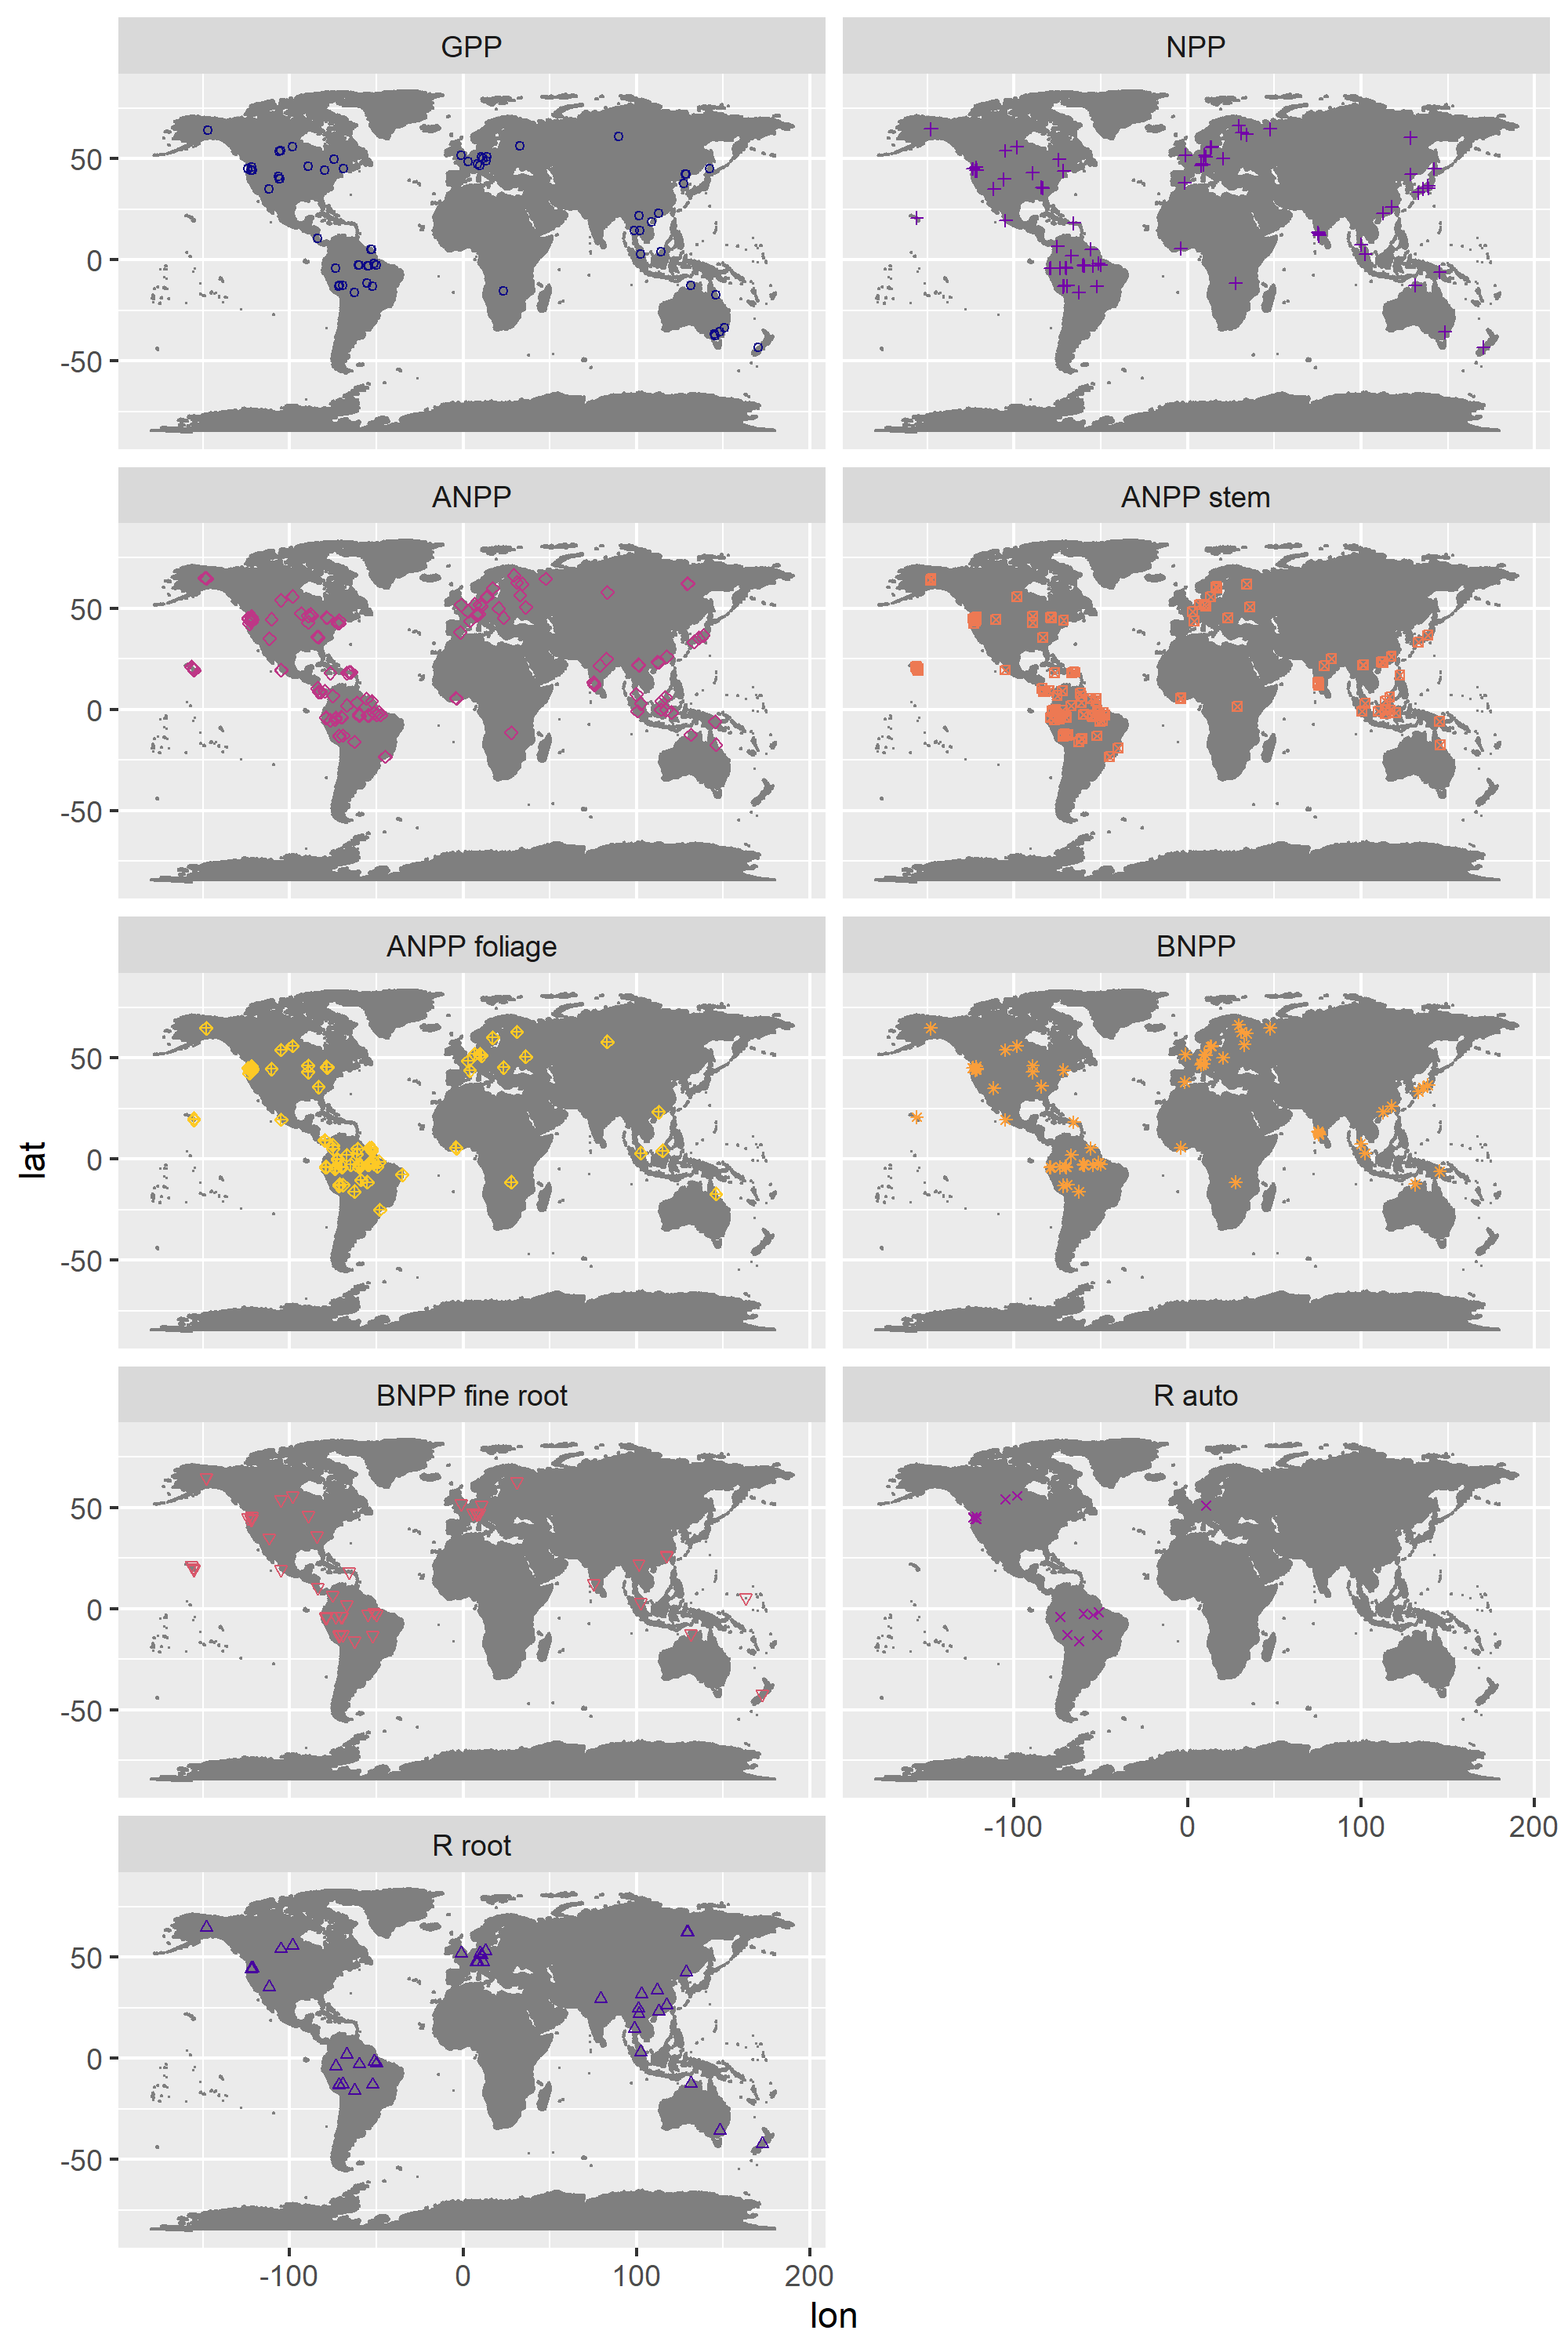
\includegraphics[height=0.95\textheight]{tables_figures/distribution_all_samples} \caption{Figure S1: Maps showing distribution of samples for the nine forest C fluxes analyzed here}\label{fig:unnamed-chunk-9}
\end{figure}

\begin{landscape}
\begin{figure}[H]

{\centering 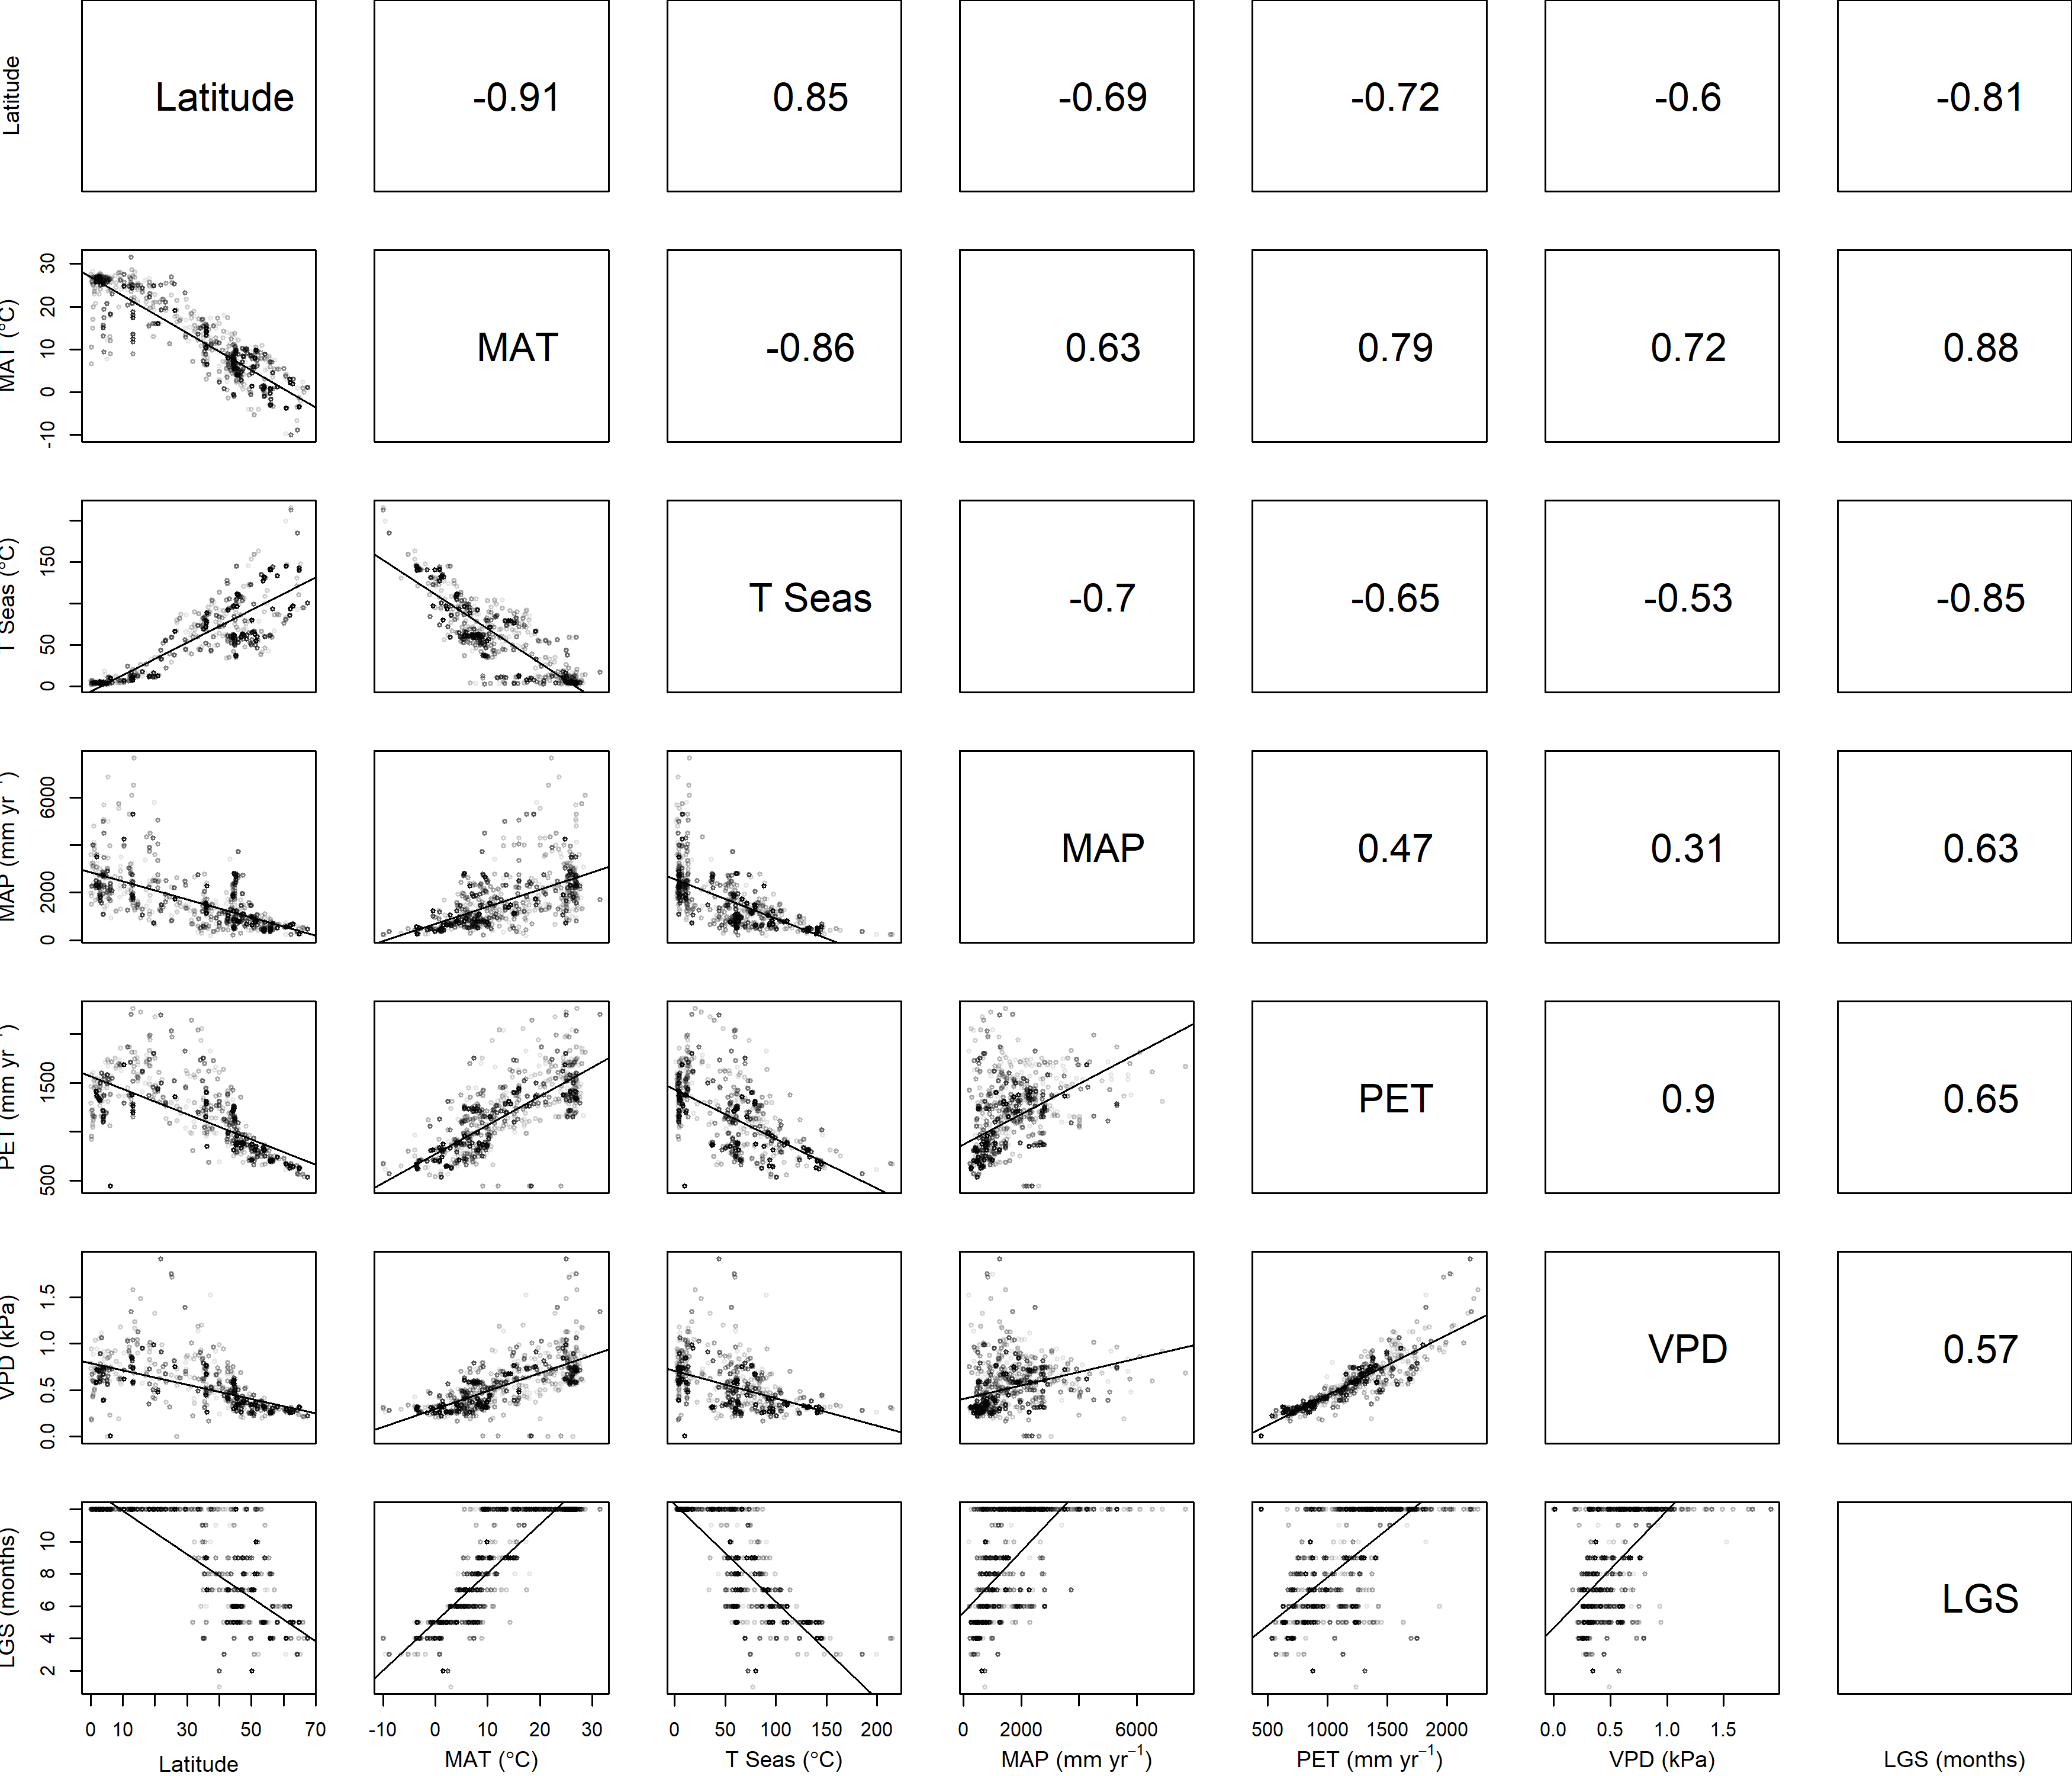
\includegraphics[height=0.95\textheight]{tables_figures/climate_regressions} 

}

\caption{Figure S2: Scatterplots and Pearson's R values for relationships between latitude and climate variables}\label{fig:unnamed-chunk-10}
\end{figure}
\end{landscape}

\begin{landscape}
\begin{figure}[H]

{\centering 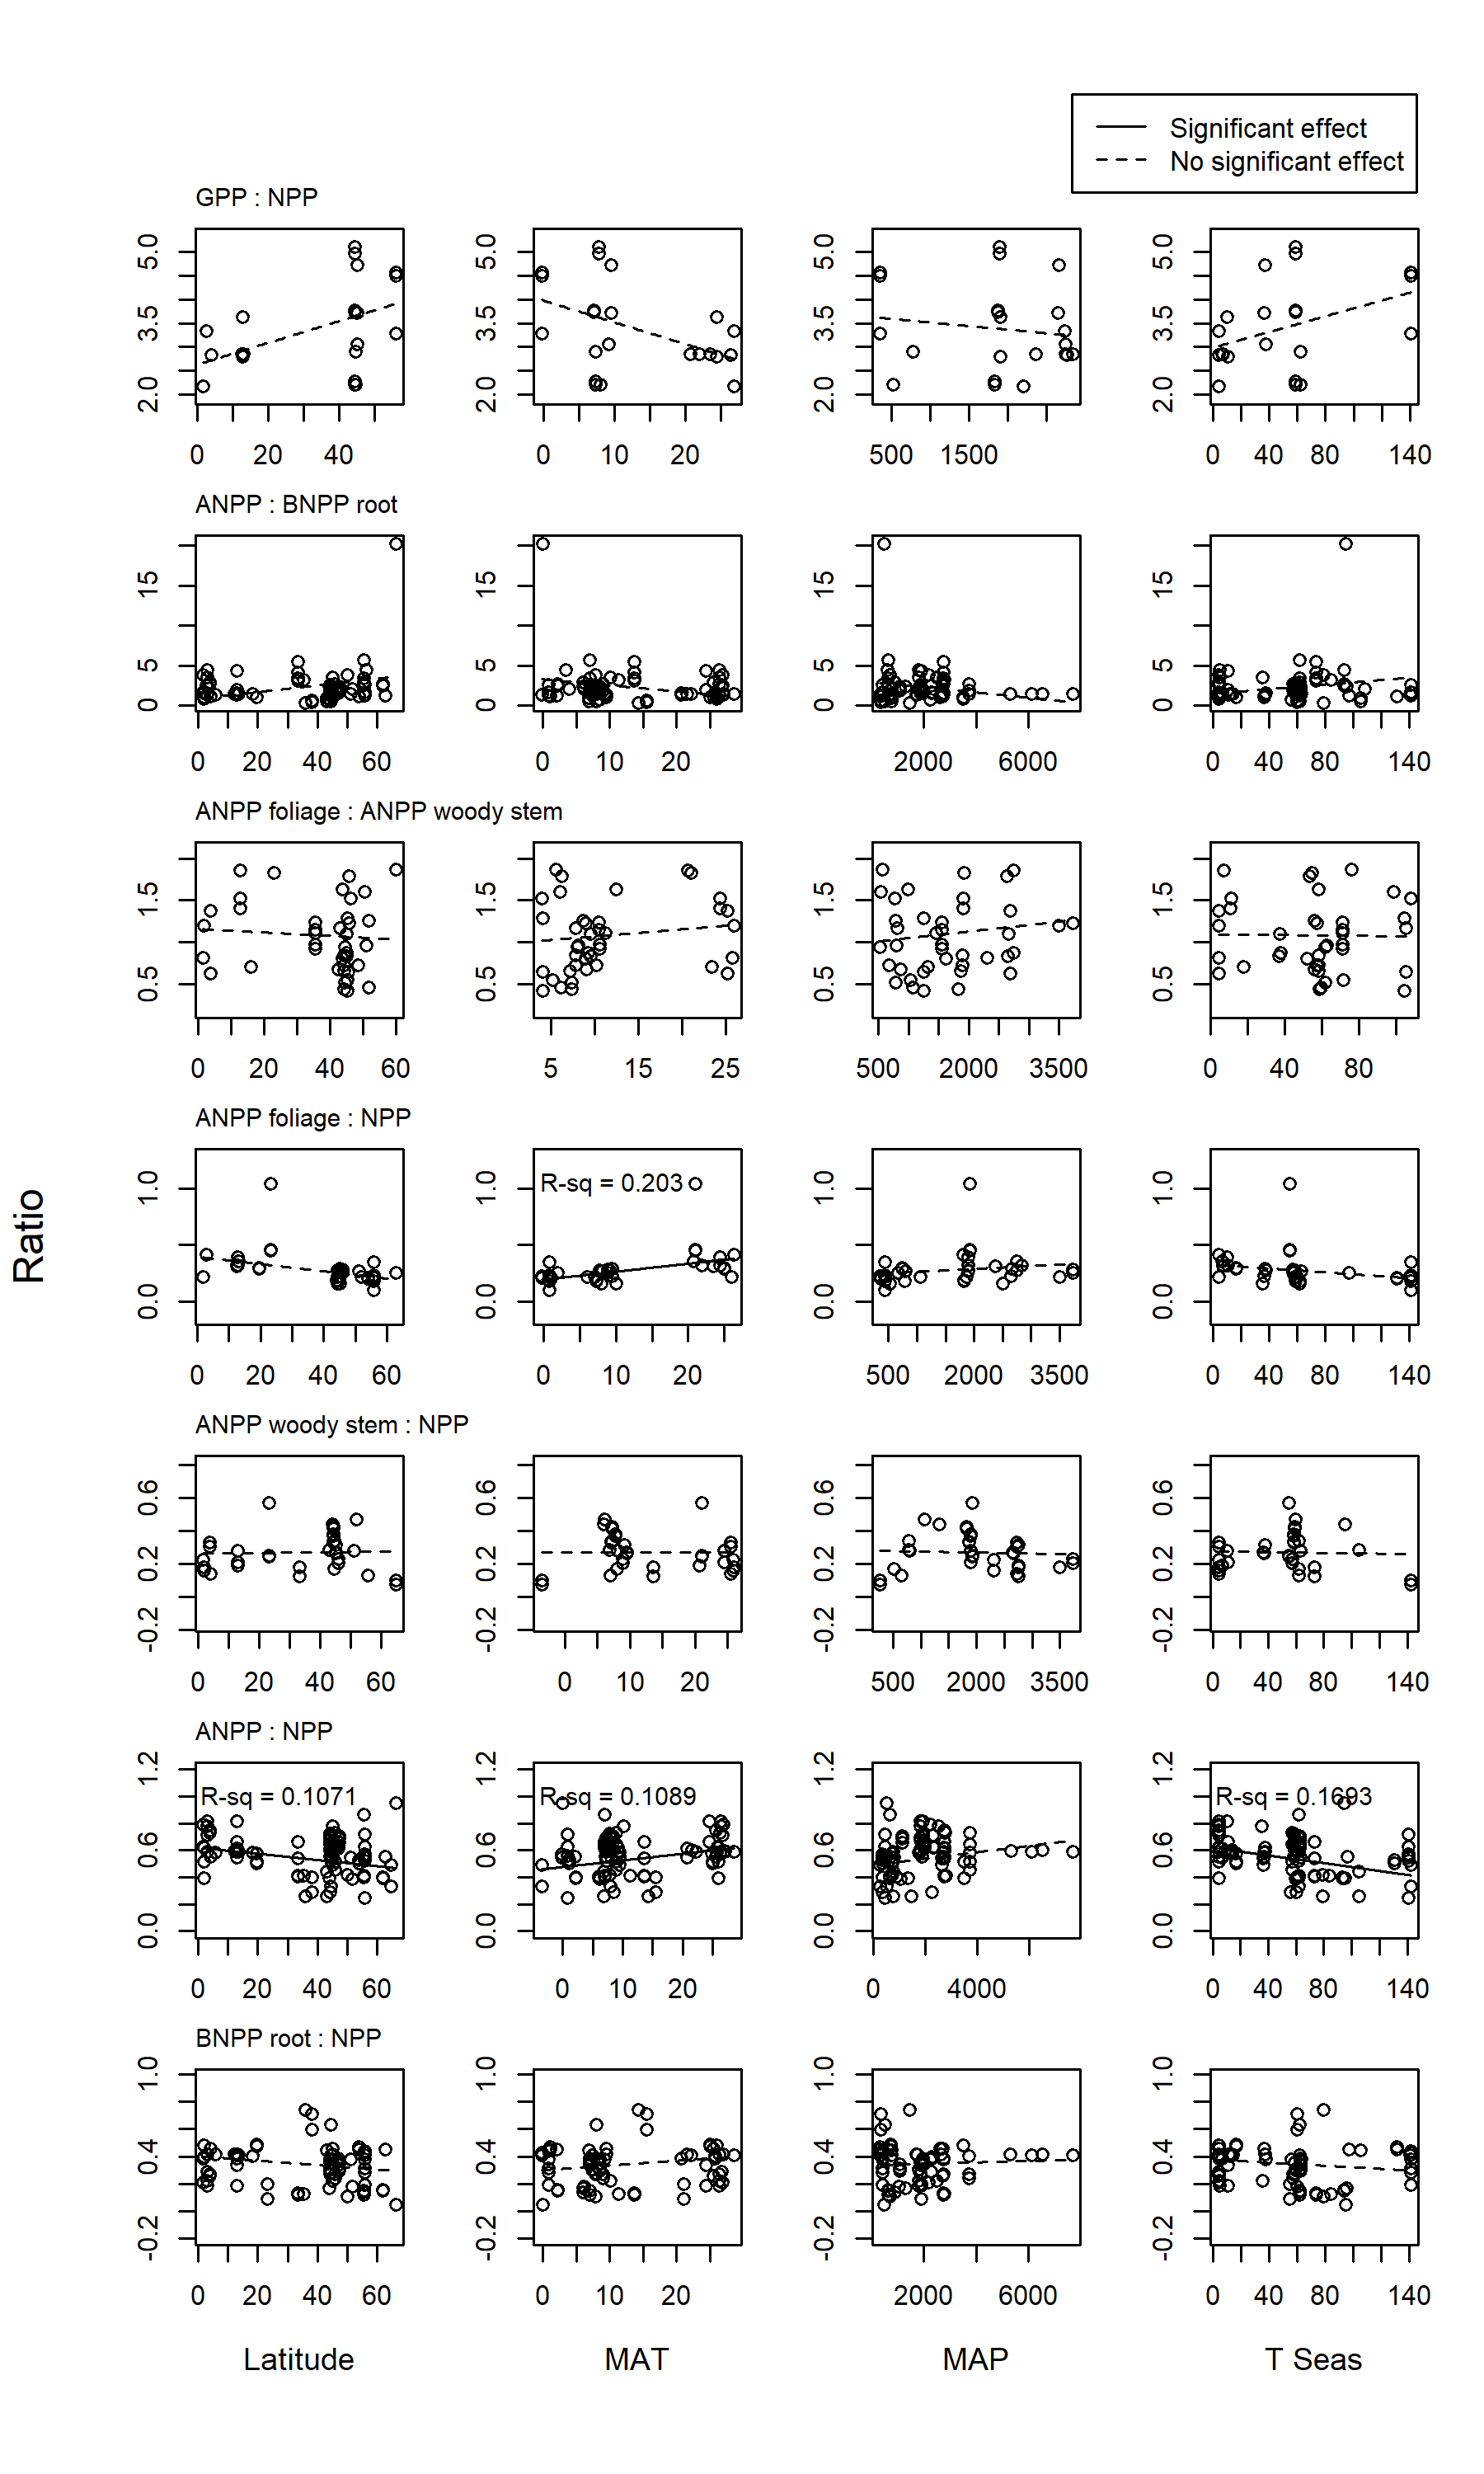
\includegraphics[width=0.8\linewidth]{tables_figures/ratio_grid_plots} 

}

\caption{Figure S3: Ratios among forest C fluxes as a function of latitude and climate variables}\label{fig:unnamed-chunk-11}
\end{figure}
\end{landscape}

\begin{landscape}
\begin{figure}[H]
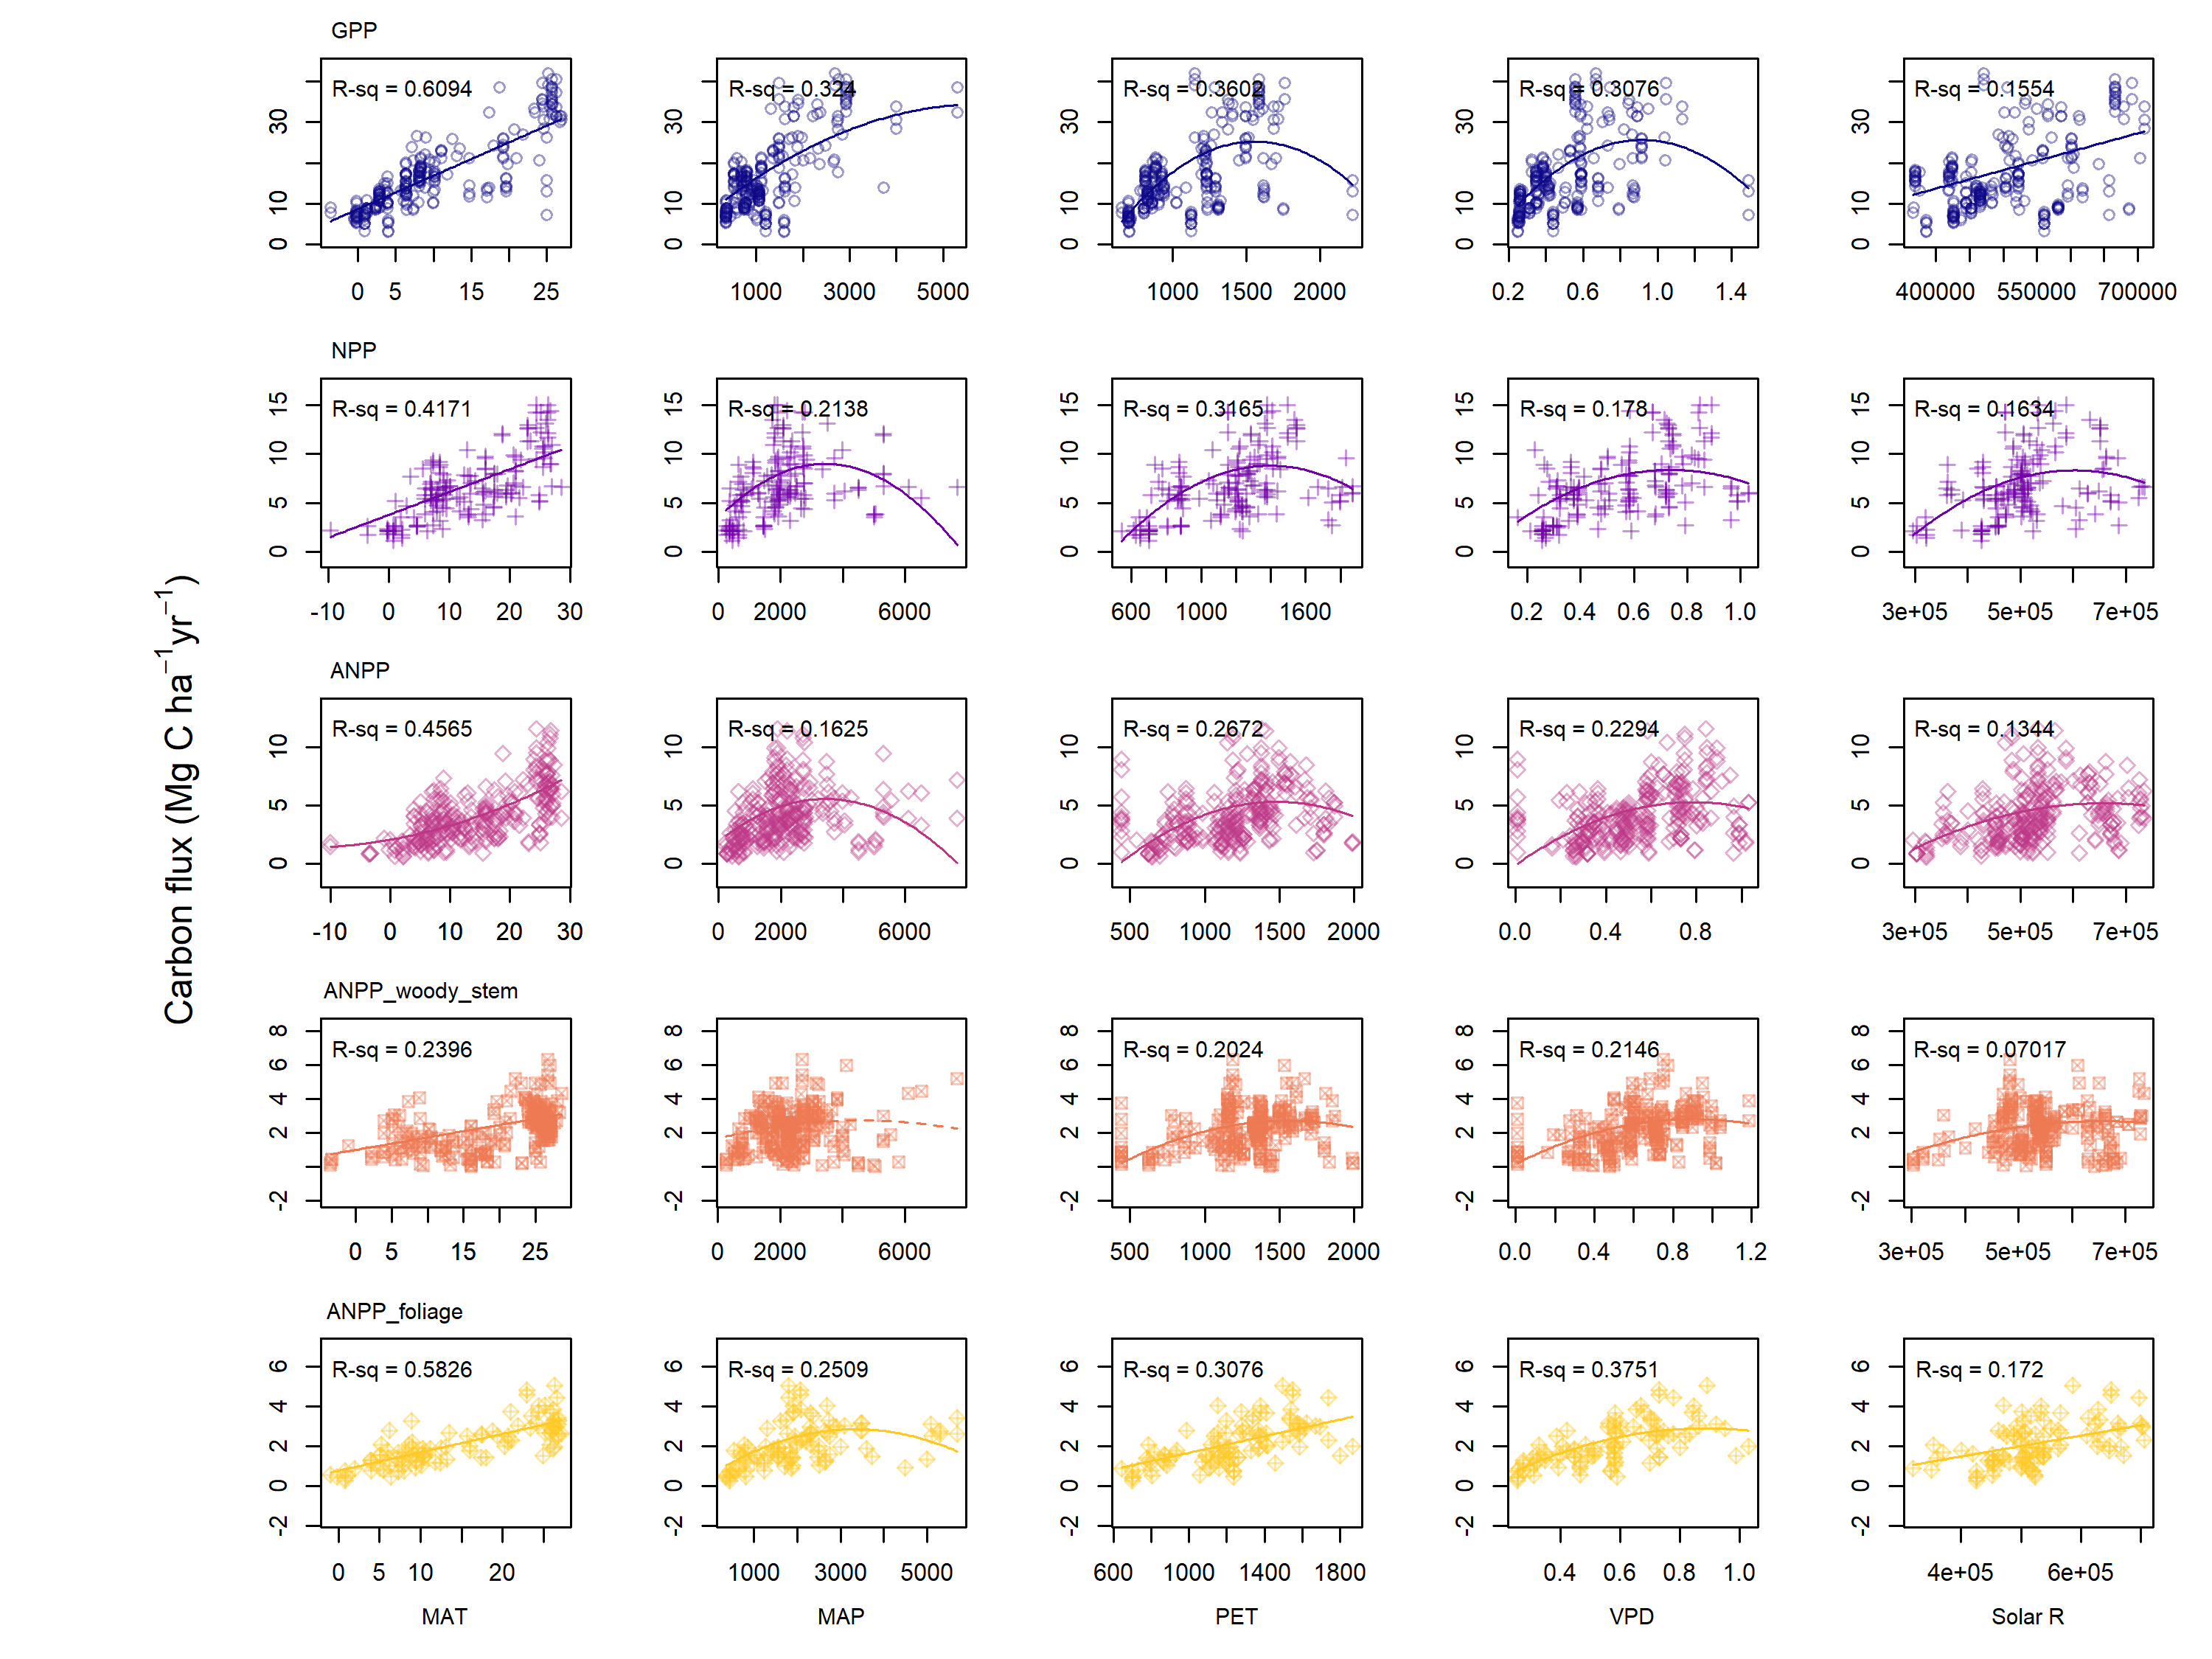
\includegraphics[height=0.95\textheight]{tables_figures/grid_plots_climate1} \caption{Figure S4: Individual plots of forest C fluxes in relation to mean annual climate, part 1.}\label{fig:unnamed-chunk-12}
\end{figure}

\newpage

\begin{figure}[H]
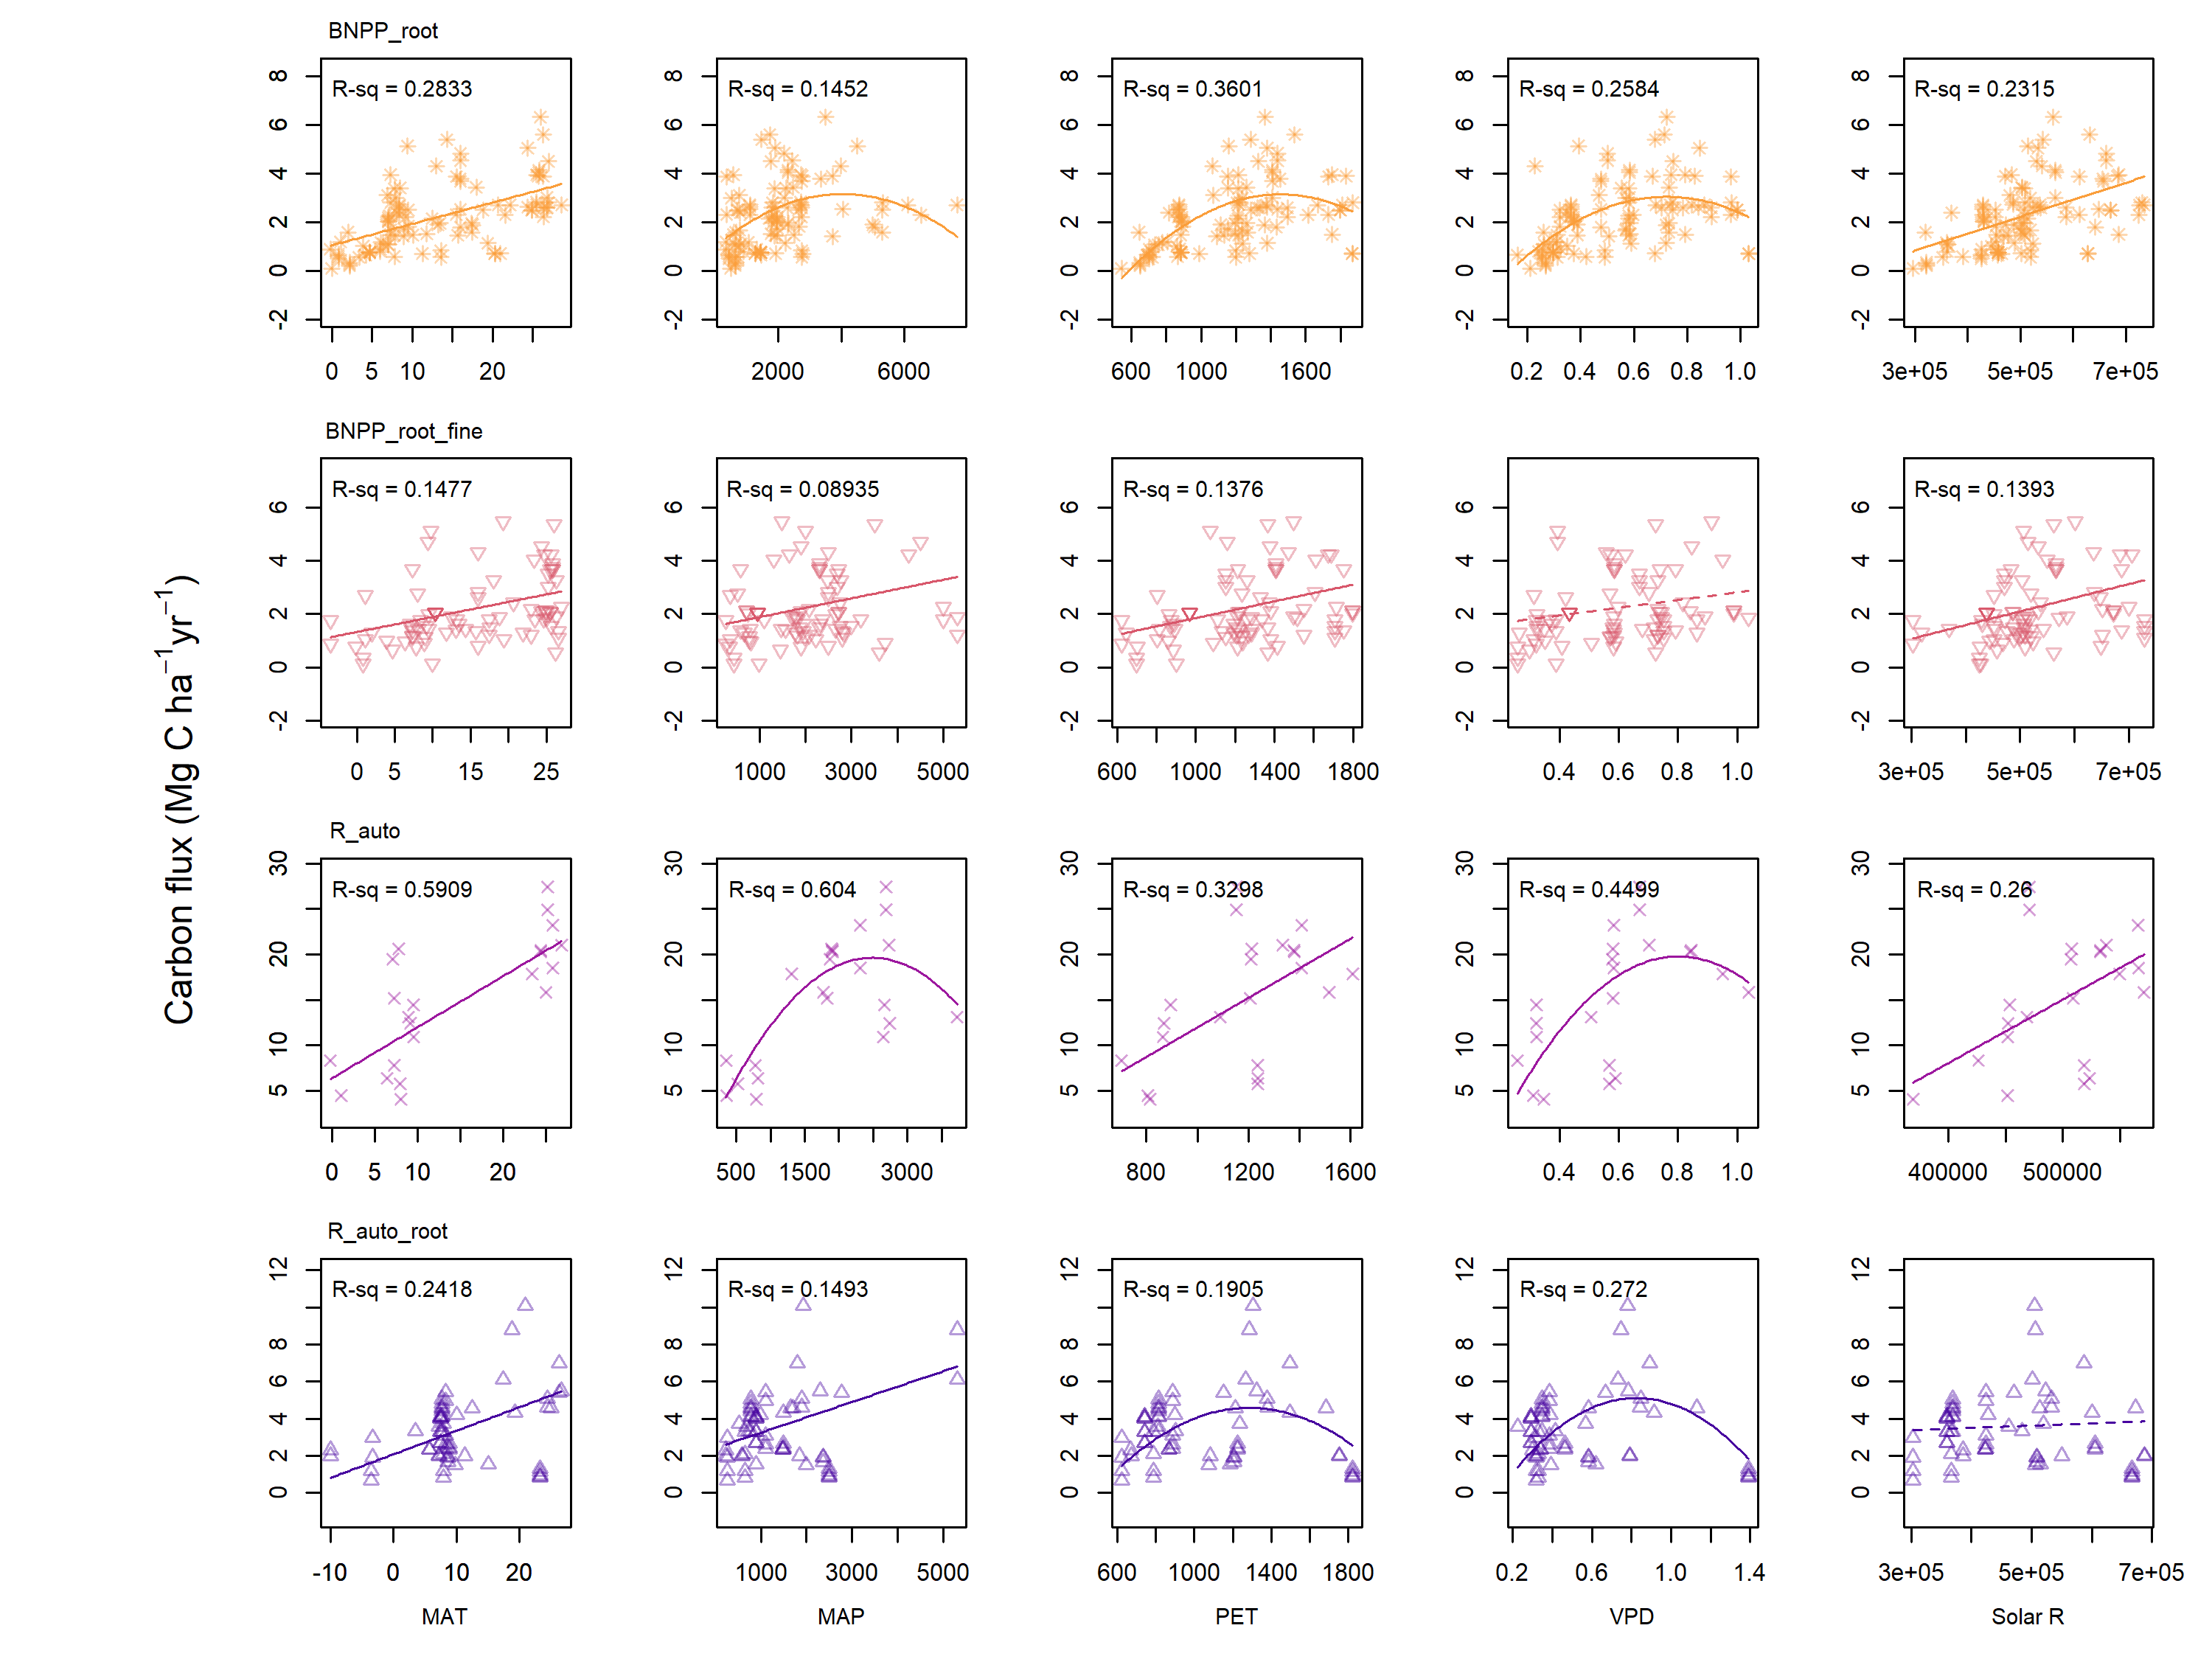
\includegraphics[height=0.95\textheight]{tables_figures/grid_plots_climate2} \caption{Figure S5: Individual plots of forest C fluxes in relation to mean annual climate, part 2.}\label{fig:unnamed-chunk-13}
\end{figure}
\end{landscape}

\begin{figure}[H]
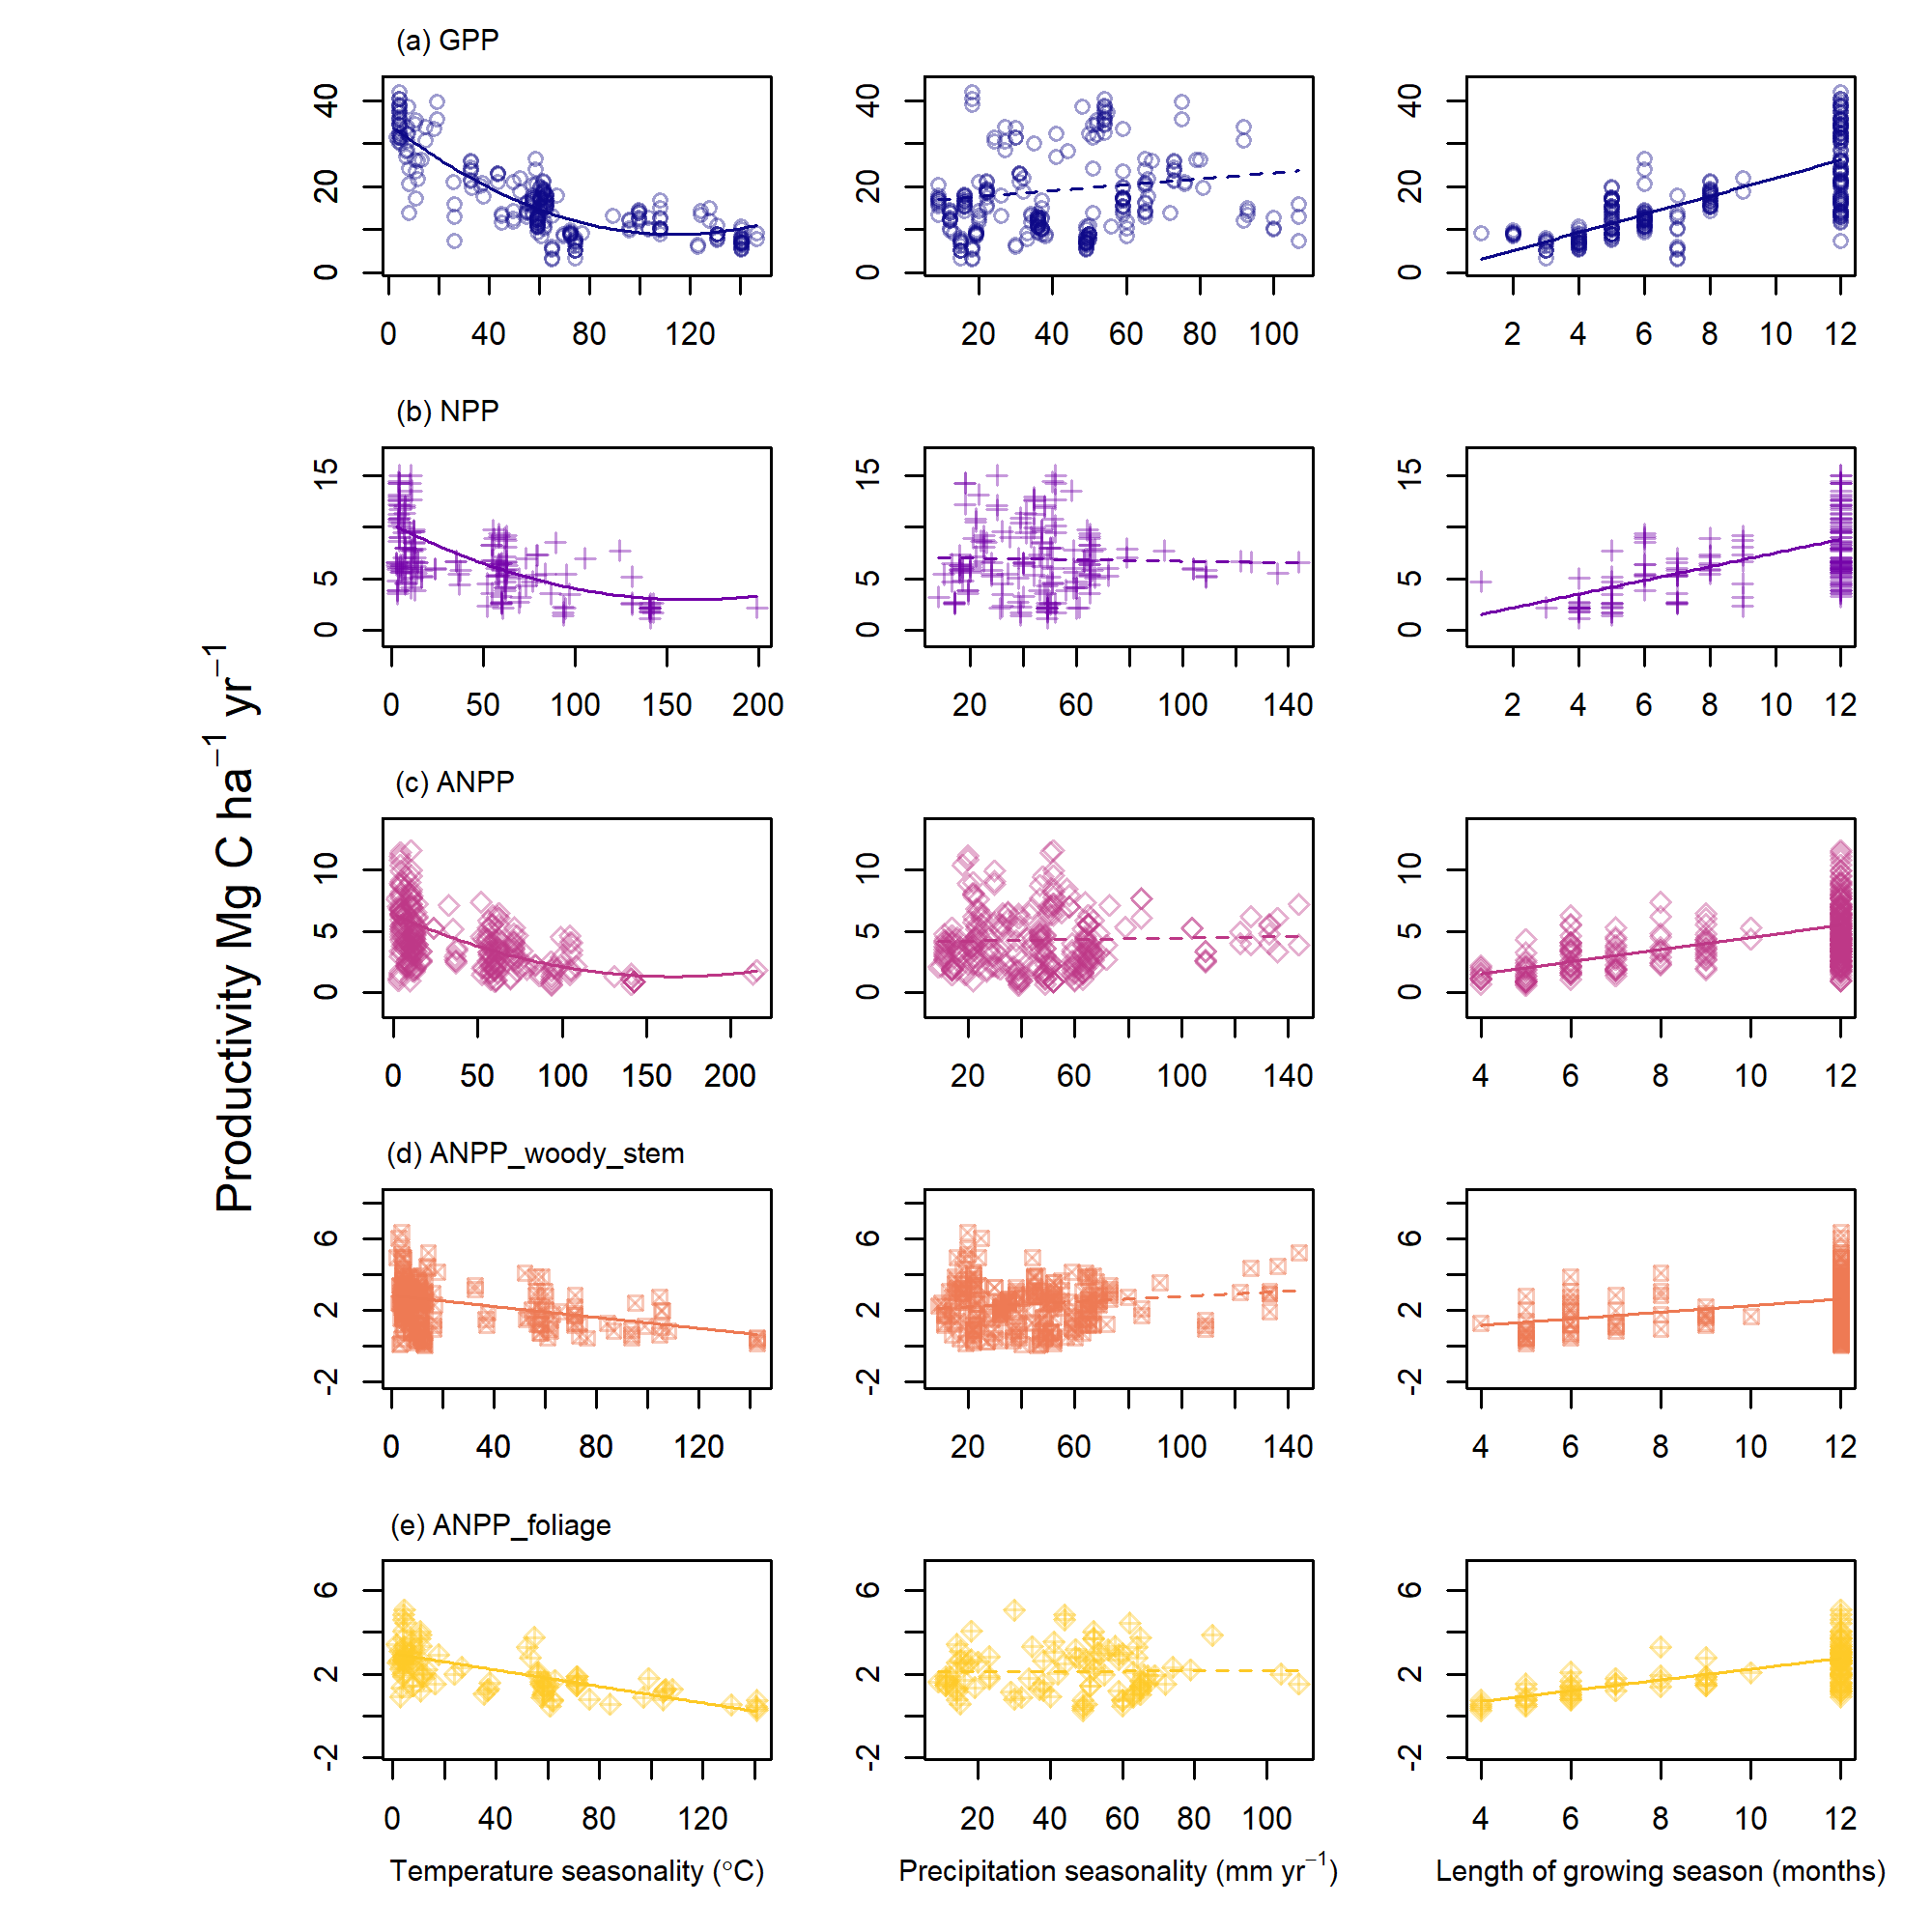
\includegraphics[height=0.95\textheight]{tables_figures/grid_plots_seasonality3} \caption{Figure S6: Individual plots of forest C fluxes in relation to mean climate seasonality, part 1.}\label{fig:unnamed-chunk-14}
\end{figure}

\newpage
\begin{figure}[H]
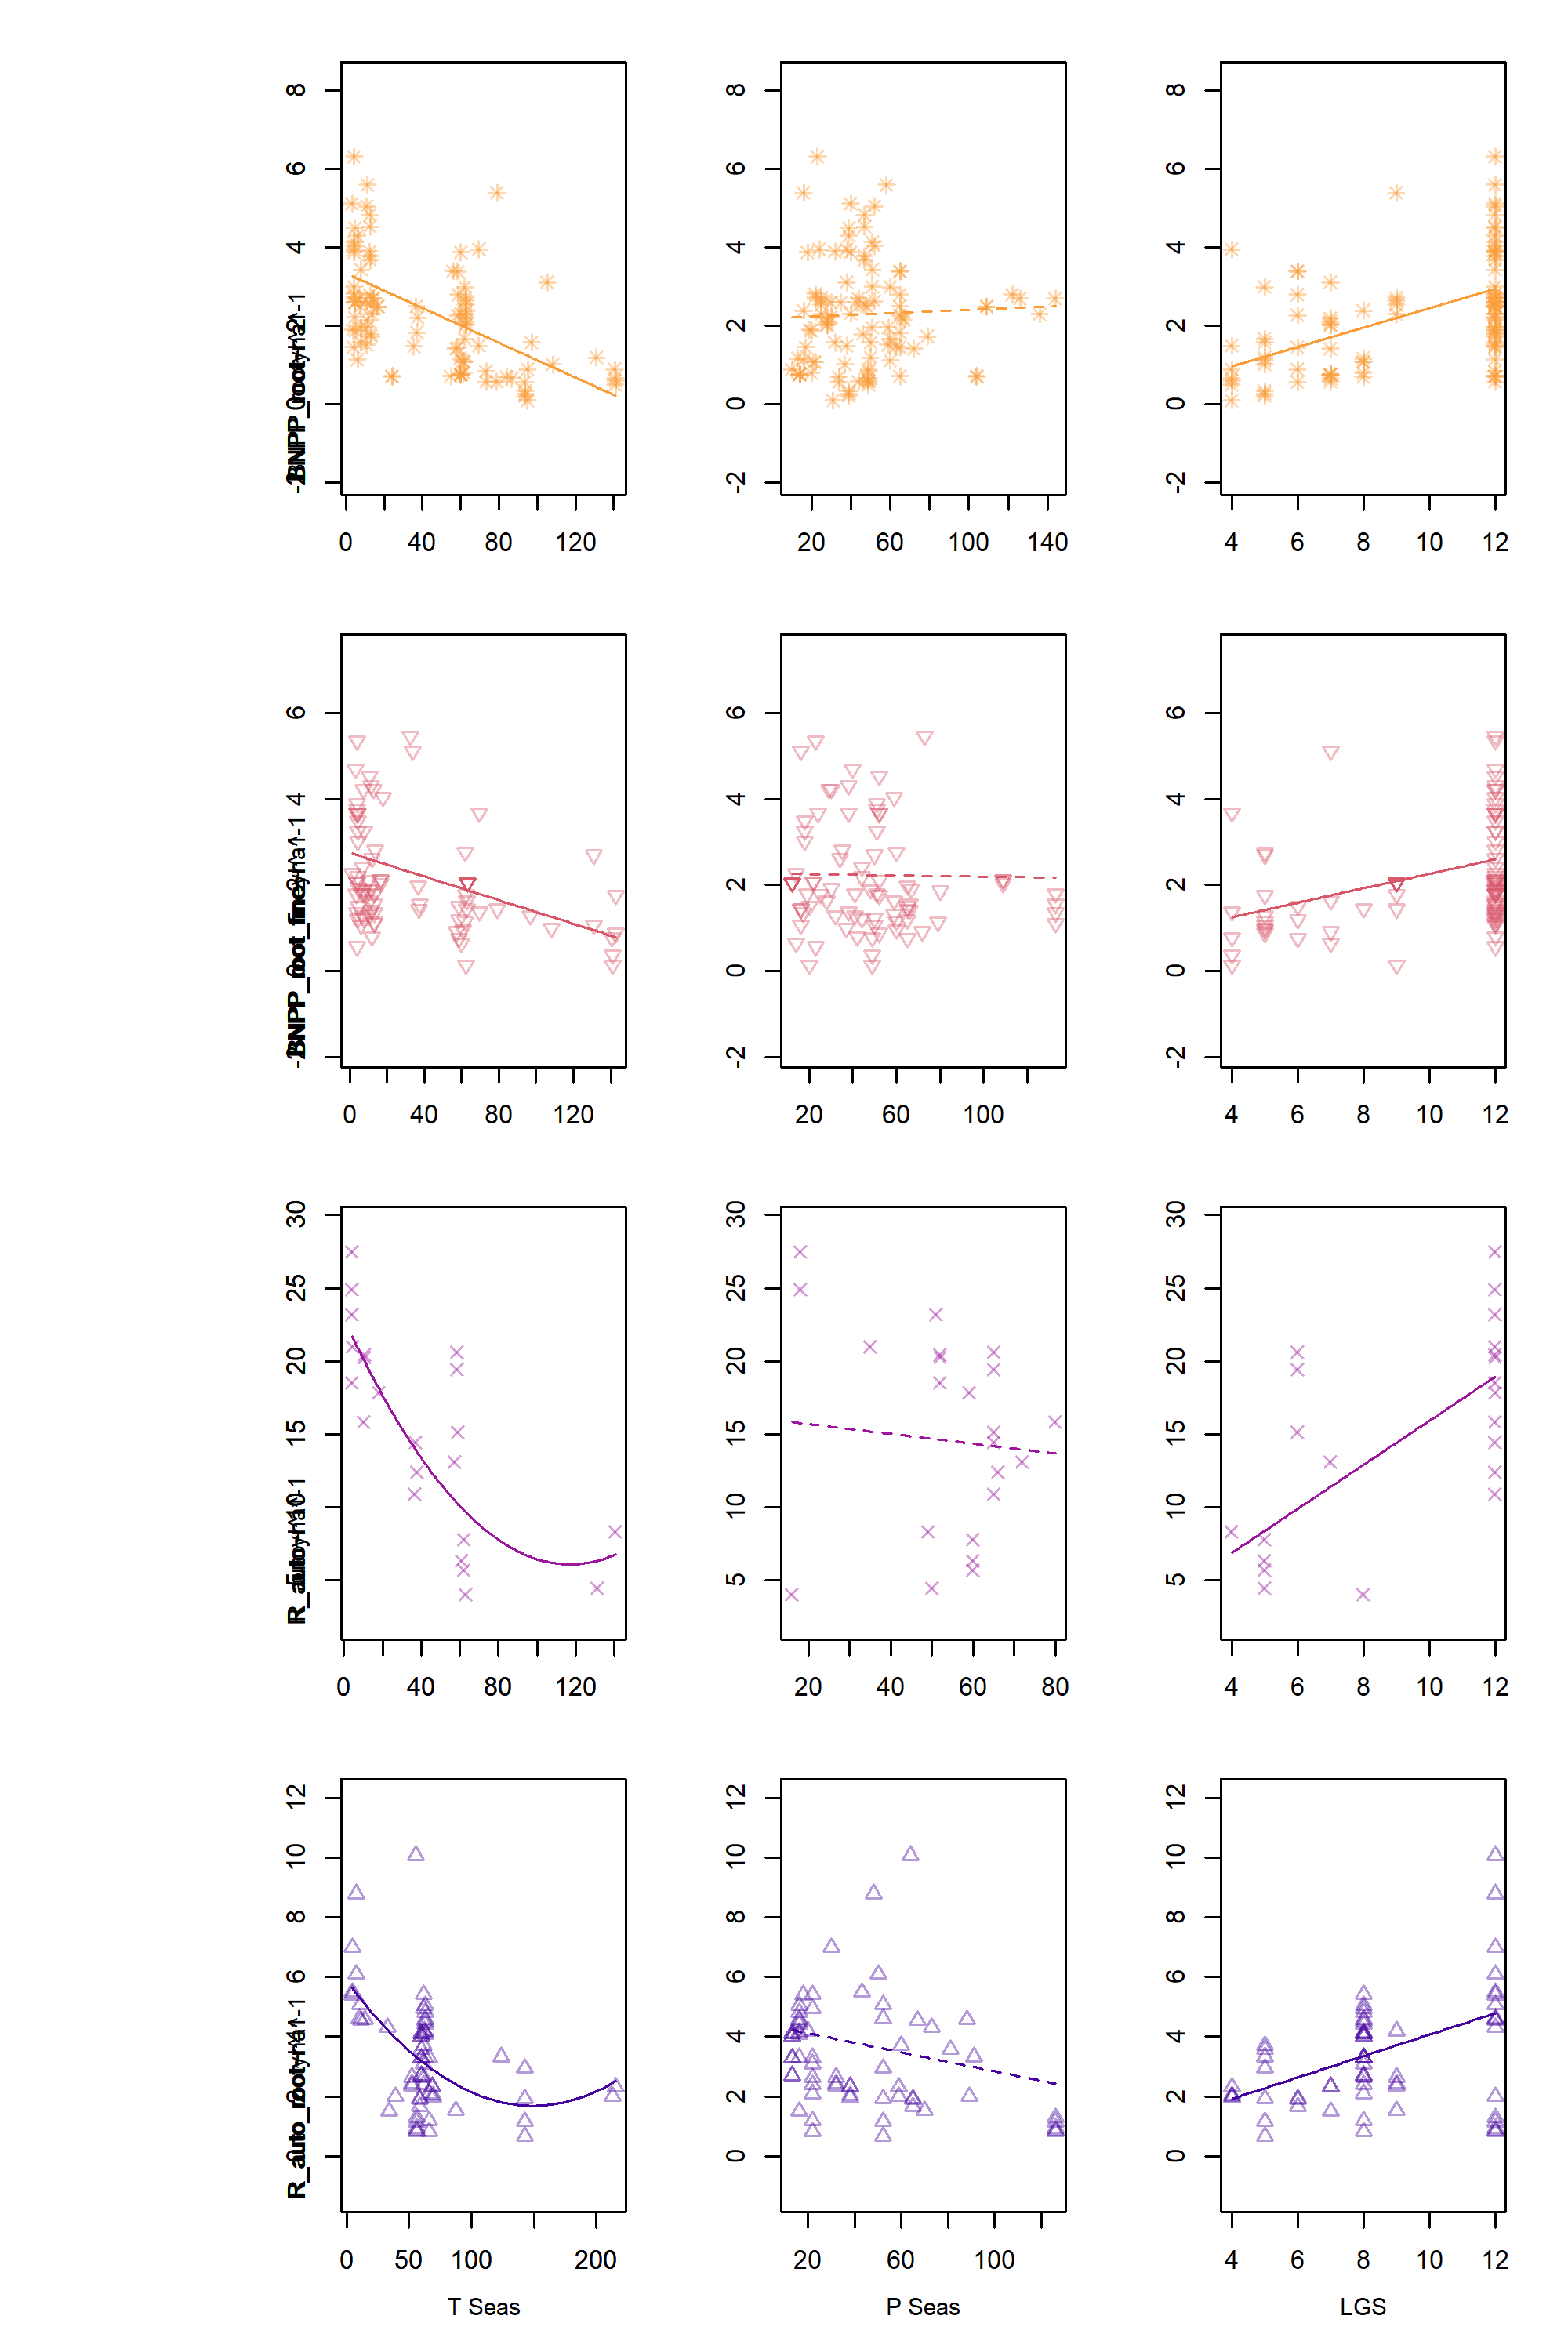
\includegraphics[width=1\linewidth]{tables_figures/grid_plots_seasonality4} \caption{Figure S7: Individual plots of forest C fluxes in relation to mean climate seasonality, part 2.}\label{fig:unnamed-chunk-15}
\end{figure}

\newpage
\begin{figure}[H]
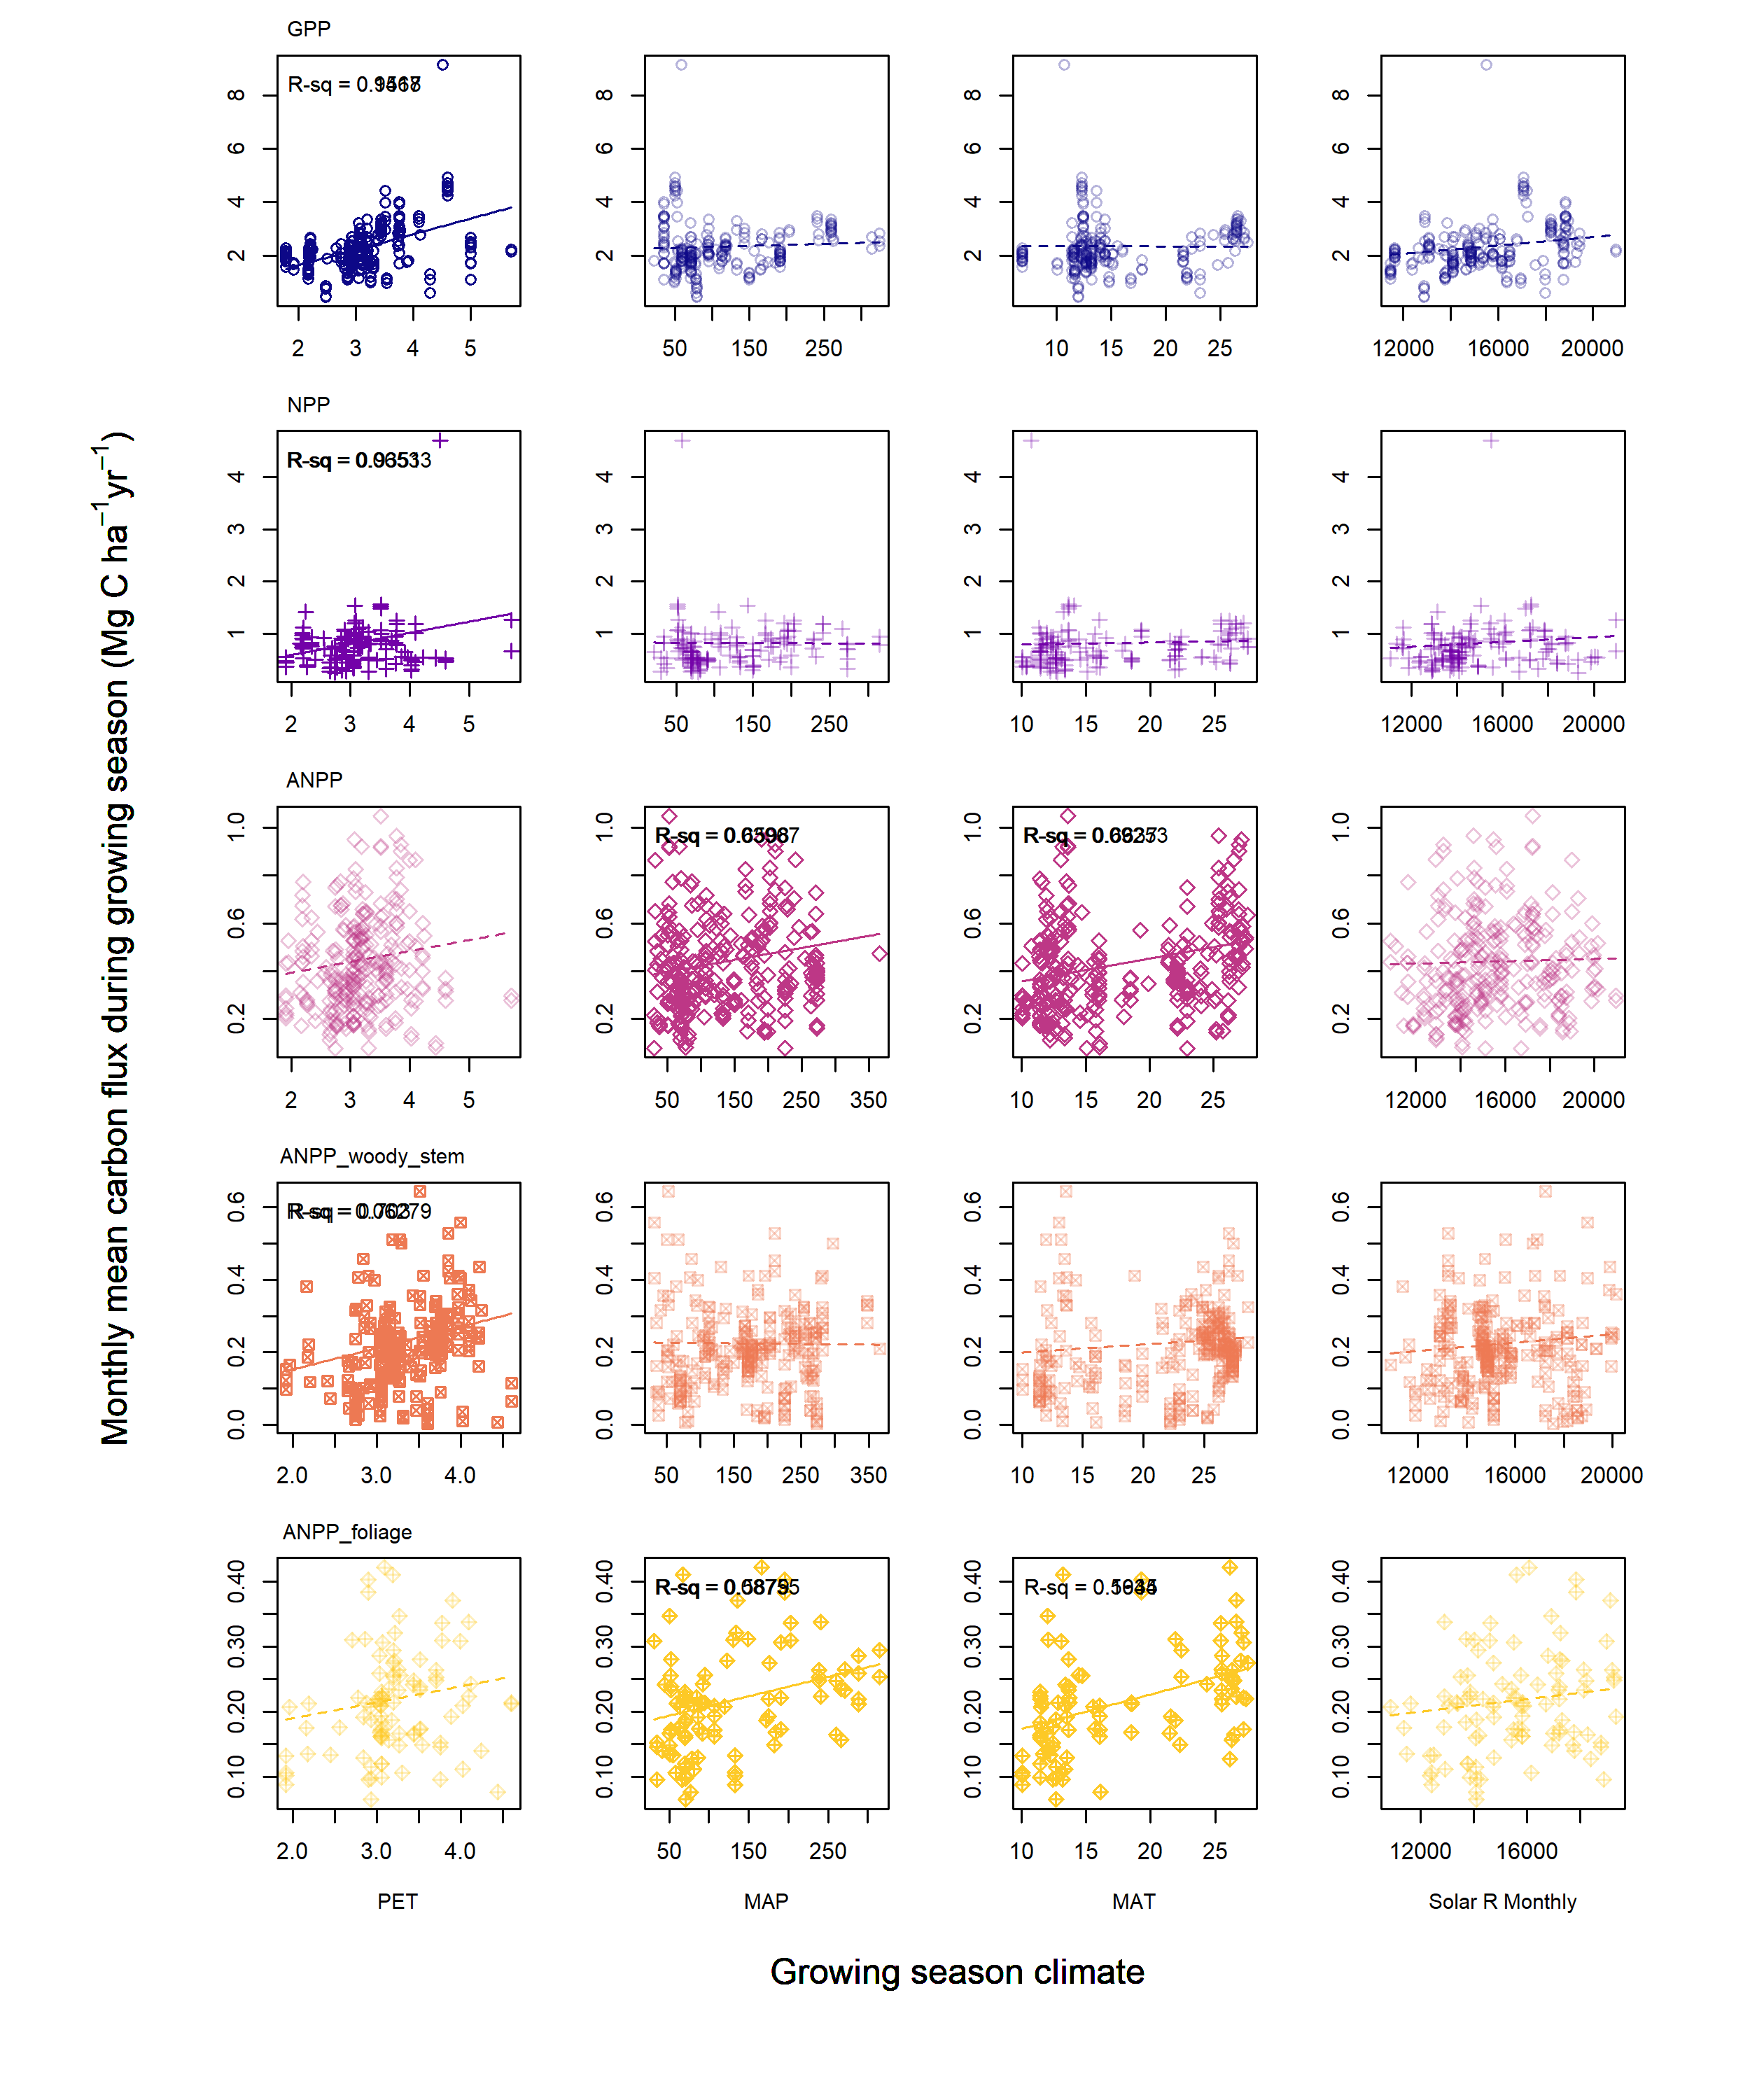
\includegraphics[width=1\linewidth]{tables_figures/gridded_growing_season1} \caption{Figure S8: Growing season length-standardized forest C fluxes in relation to mean growing season climate, part 1.}\label{fig:unnamed-chunk-16}
\end{figure}

\newpage
\begin{figure}[H]
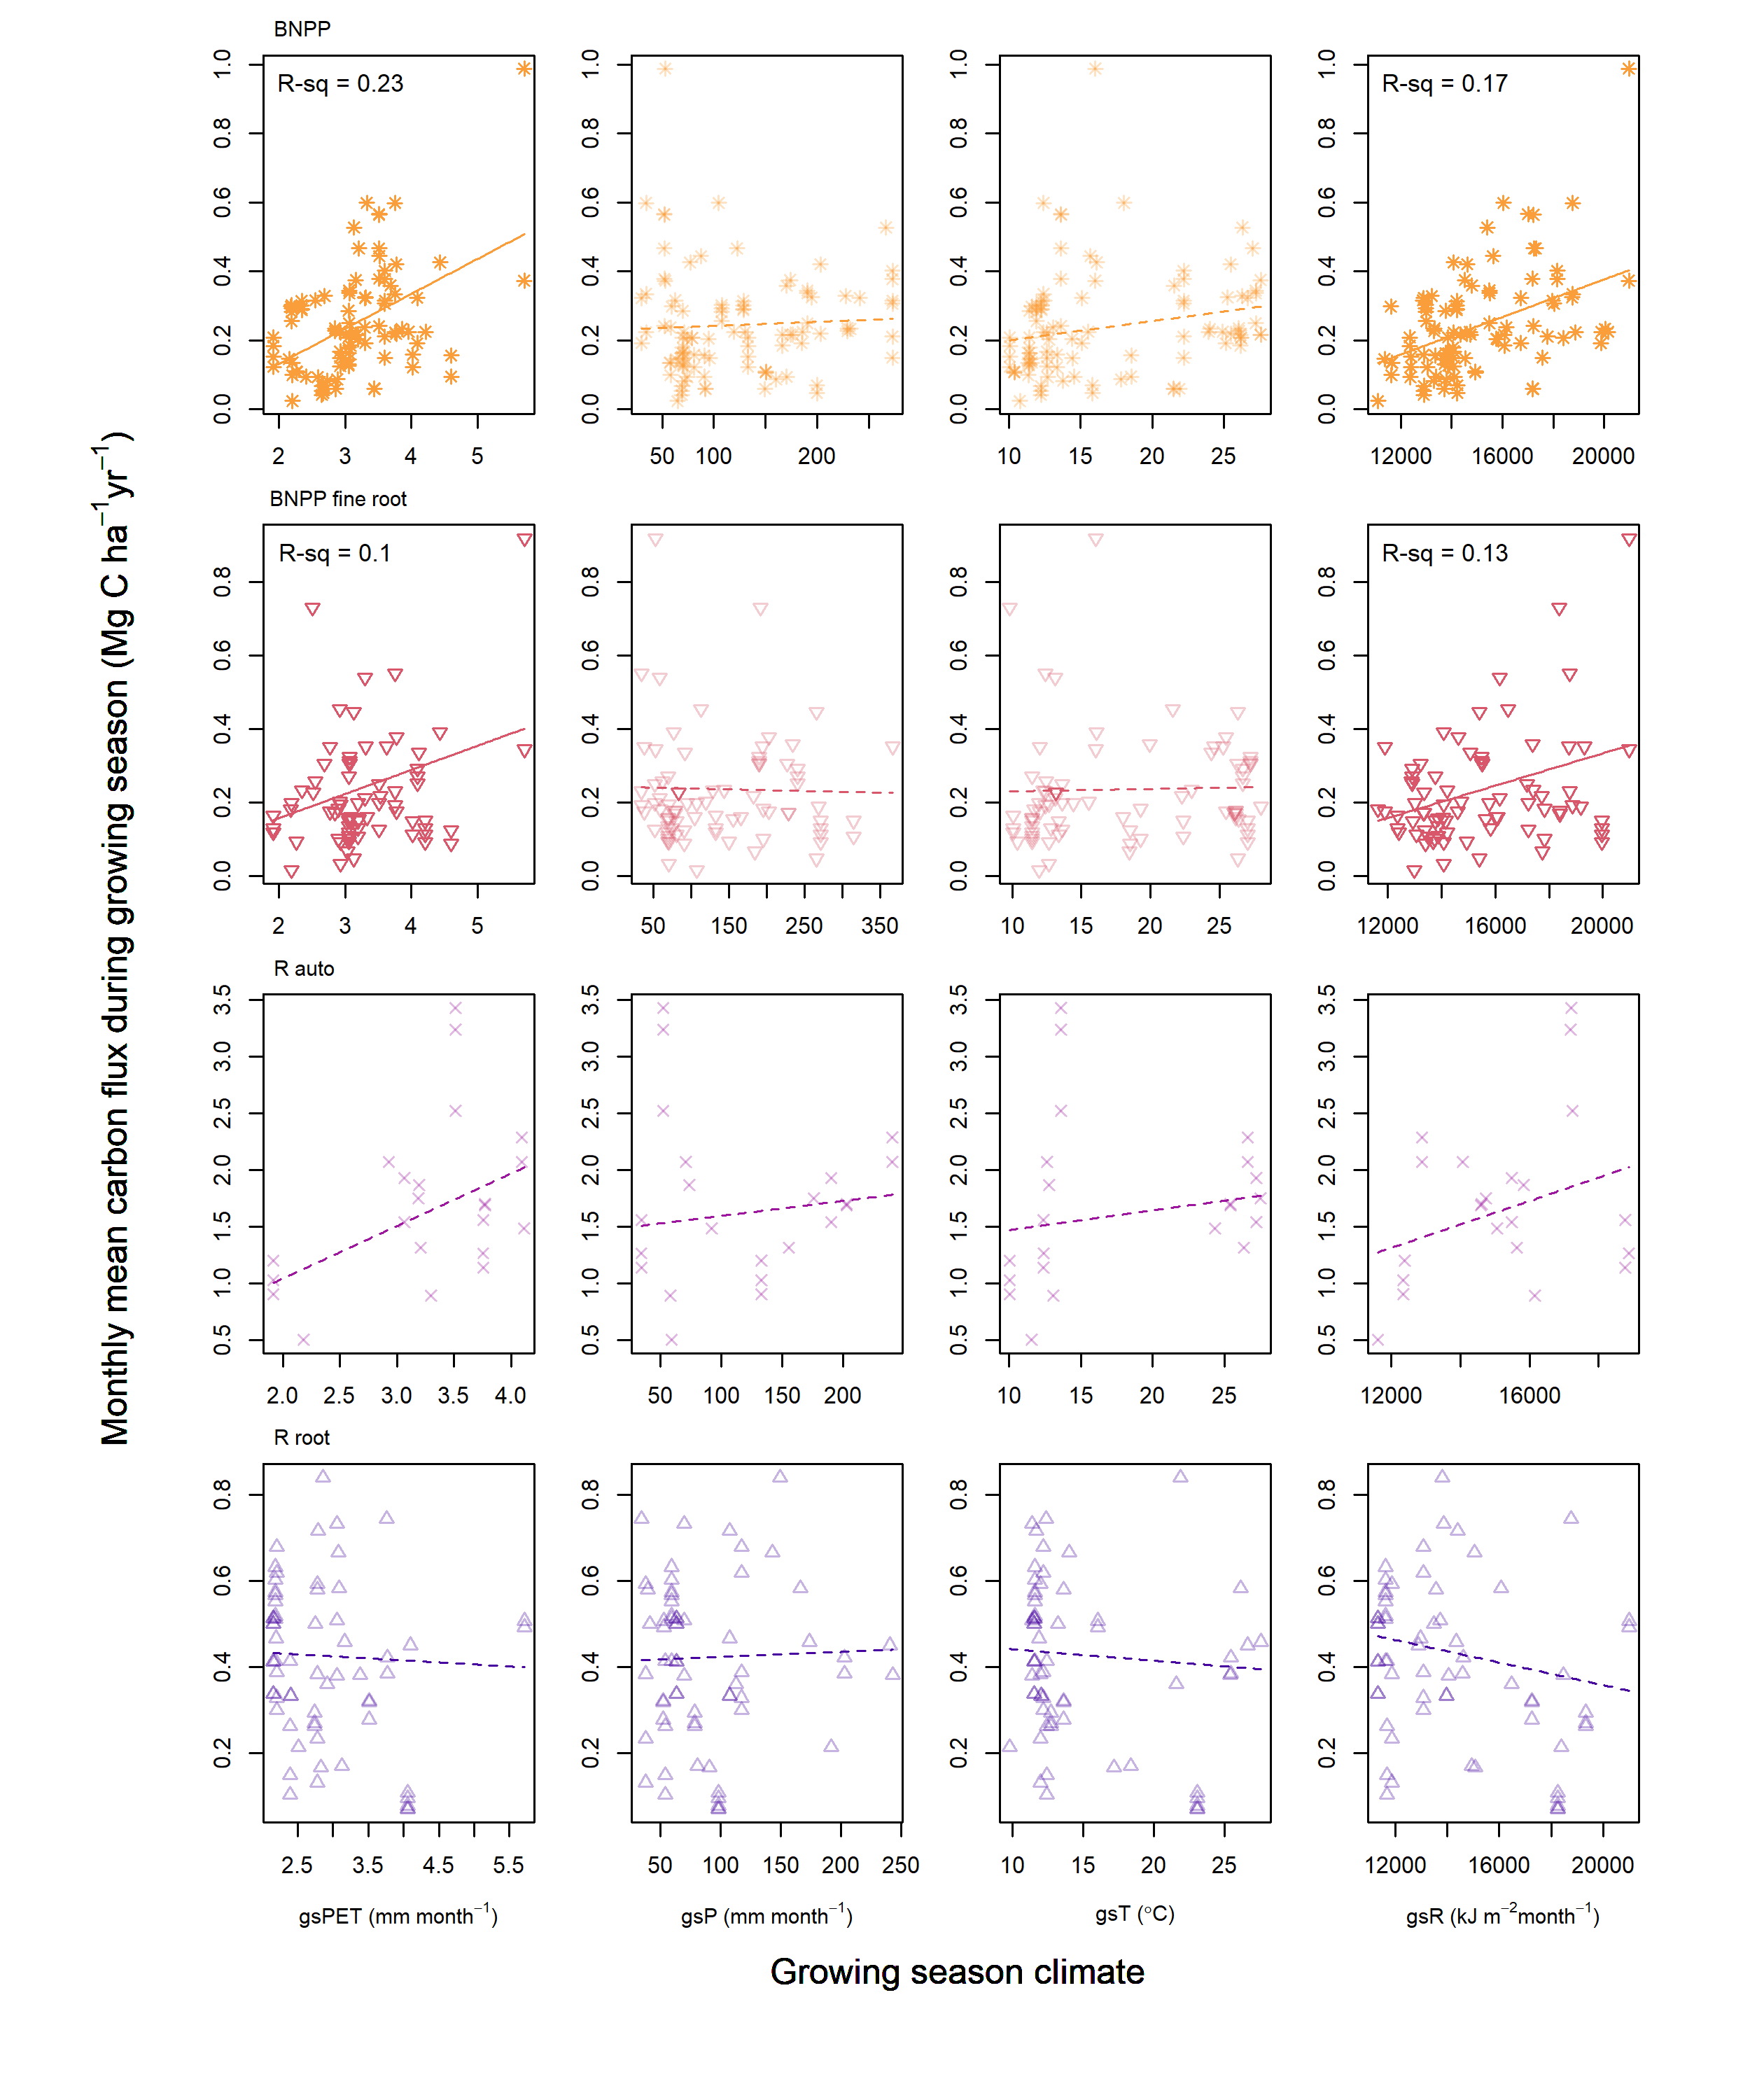
\includegraphics[width=1\linewidth]{tables_figures/gridded_growing_season2} \caption{Figure S9: Growing season length-standardized forest C fluxes in relation to mean growing season climate, part 2.}\label{fig:unnamed-chunk-17}
\end{figure}

\newpage

\hypertarget{references}{%
\section*{References}\label{references}}
\addcontentsline{toc}{section}{References}

\hypertarget{refs}{}
\leavevmode\hypertarget{ref-abatzoglou_terraclimate_2018}{}%
Abatzoglou, J. T., Dobrowski, S. Z., Parks, S. A., \& Hegewisch, K. C.
(2018). TerraClimate, a high-resolution global dataset of monthly
climate and climatic water balance from 1958--2015. \emph{Scientific
Data}, \emph{5}, 170191. \url{https://doi.org/10.1038/sdata.2017.191}

\leavevmode\hypertarget{ref-fick_worldclim_2017}{}%
Fick, S. E., \& Hijmans, R. J. (2017). WorldClim 2: New 1-km spatial
resolution climate surfaces for global land areas. \emph{International
Journal of Climatology}, \emph{37}(12), 4302--4315.
\url{https://doi.org/10.1002/joc.5086}

\leavevmode\hypertarget{ref-harris_updated_2014}{}%
Harris, I., Jones, P. D., Osborn, T. J., \& Lister, D. H. (2014).
Updated high-resolution grids of monthly climatic observations - the CRU
TS3.10 dataset: \emph{International Journal of Climatology},
\emph{34}(3), 623--642. \url{https://doi.org/10.1002/joc.3711}

\leavevmode\hypertarget{ref-hijmans_very_2005}{}%
Hijmans, R. J., Cameron, S. E., Parra, J. L., Jones, P. G., \& Jarvis,
A. (2005). Very high resolution interpolated climate surfaces for global
land areas. \emph{International Journal of Climatology}, \emph{25}(15),
1965--1978. \url{https://doi.org/10.1002/joc.1276}

\end{document}
